\chapter{优化问题与解}
\label{chap:optimization}

想象手里有一张地形图，任务是找到最低的地方。图上有些区域禁止进入，只有一块“允许站的地”；地面高度由某个规则给出，我们能逐点查到。这件事听起来简单，真做起来却会遇到一串问题：允许站的地可能根本不存在；地面可能一路向下延伸，没有底；也可能越走越低，却总差一步才到最低处。即使最低点存在，它也许不止一个；站在某个洼地底部向四周看处处更高，却不知道山那边有没有更深的谷。最后，我们实际交出的总是一个“差不多”的位置，还要说清它离真正的最低点有多远、为它花了多少计算。

本章把这幅画面变成数学。地形图上的位置是决策变量，允许站的地是可行域，地面高度是目标函数；找最低点就是求解优化问题。两个具体任务贯穿全章：一个车间在工时和原料的限制下安排两种产品的产量，使利润最大；一组观测数据用带正则项的最小二乘拟合参数。前者的可行域是一块有棱角的多边形，后者的可行域是整个空间，目标却是一只可能很扁的“碗”。学习目标是：能把一个任务写成完整的优化问题，说清“解”指什么、何时存在、何时唯一、怎样用导数判别，并在不预设任何算法已经成功的前提下，规定评价近似解好坏和计算代价的共同语言。

各节的顺序由这些问题的依赖关系决定。先把问题写完整，才能定义最优值与最优解，并区分只与附近比较的局部最优；扩展实值写法把约束并入目标，使后面的论证只需处理一个函数。有了“解”的定义，下一步问它是否存在：这需要最小化序列留在有界区域、极限仍然可行、目标值的比较能传到极限。存在之后，凸性回答“局部最优是否就是全局最优”，严格凸与强凸进一步回答“解是否唯一”“目标差能否换成到解的距离”。光滑目标的一阶、二阶条件把这些几何性质翻译成可以逐点检查的梯度与Hessian判据。最后，由于实际计算只能交出近似解，我们规定用哪些误差衡量它，以及怎样把迭代轮数与每轮代价合成为总计算成本。本章不讲任何迭代算法；怎样产生越来越好的候选，是后续各章的任务。

\section{优化问题的表述}
\label{sec:opt-prob-formulation}

要找“最低点”，先得说清在哪些位置里找、按什么高度比较。本节先规定一个优化问题由哪些对象组成，再定义最优值与最优解，并区分只和附近比较的局部最优与和所有候选比较的全局最优。最后引入扩展实值写法，把“哪些位置允许站”并入目标函数本身；这种写法只统一表示方式，不改变问题的解。

\subsection{变量、目标与可行域}
\label{sec:opt-prob-variables}

\paragraph{资源分配}
一个车间生产两种产品，产量分别记为$x_1,x_2$（单位：批）。每批产品一的利润为$3$，产品二为$2$。生产受两种资源限制：每批产品各用$1$个工时，每天共有$4$个工时；每批产品一用$2$份原料、产品二用$1$份，每天共有$6$份原料。产量不能为负。可以调整的量是$\bm x=(x_1,x_2)^\top\in\mathbb R^2$，要比较的是利润$3x_1+2x_2$，允许的产量组合满足
\begin{equation}
  x_1+x_2\leq4,\qquad 2x_1+x_2\leq6,\qquad x_1\geq0,\qquad x_2\geq0.
  \label{eq:opt-prob-resource}
\end{equation}
一般地，$d$种产品、$m$种资源时，变量是$\bm x\in\mathbb R^d$，利润系数$\bm c\in\mathbb R^d$，第$i$种资源每单位产品$j$的用量为$G_{i,j}$，资源上限为$h_i$；约束写成$\bm G\bm x\leq\bm h$与$\bm x\geq\bm 0$，其中$\bm G\in\mathbb R^{m\times d}$，向量不等式逐个坐标理解。

利润要最大化，而本书统一讨论最小化。二者只差一个符号：最大化$3x_1+2x_2$与最小化$f(\bm x)=-(3x_1+2x_2)$选出相同的产量，最大利润等于最小值的相反数。一般地，$\max_{\bm x\in C}p(\bm x)=-\min_{\bm x\in C}\bigl(-p(\bm x)\bigr)$，取得两侧的点也相同。这个转换是记号上的约定，不涉及任何求解技巧。

图~\ref{fig:opt-prob-resource-region}把约束~\eqref{eq:opt-prob-resource}画在平面上：四条直线围出一个四边形，它就是“允许站的地”。虚线是利润相等的产量组合，沿箭头方向平移时利润增大。读者可以从图中看到，利润为$10$的直线恰好擦过四边形的一个角$(2,2)$，再往外移就离开了允许区域。这一观察还不是证明；第~\ref{sec:opt-prob-optimal-value}小节将给出一个两行的论证，第~\ref{chap:opt-linear-programming}章再把“在角点处寻找”发展成一般方法。

\begin{figure}[!htbp]
  \centering
  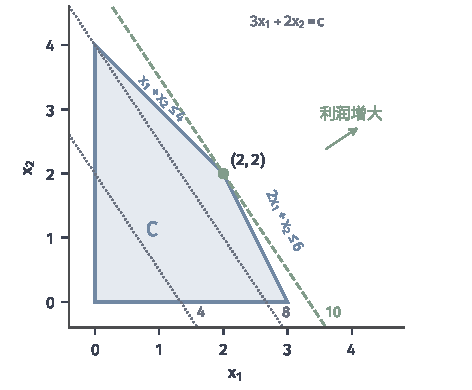
\includegraphics[width=80mm]{figures/03-optimization-evolution-and-signals/01-optimization/matplotlib/c1-resource-region/figure.pdf}
  \caption{资源分配问题的可行域与利润等值线。蓝色四边形$C$由$x_1+x_2\leq4$、$2x_1+x_2\leq6$与$\bm x\geq\bm 0$围成，顶点为$(0,0),(3,0),(2,2),(0,4)$。灰色点线与绿色虚线是$3x_1+2x_2=c$在$c=4,8,10$时的直线（数值标在横轴下方）；利润为$10$的直线只与$C$交于顶点$(2,2)$。}
  \label{fig:opt-prob-resource-region}
\end{figure}

\paragraph{带正则项的最小二乘}
第二个任务来自数据拟合。设有$n$个观测、$d$个待定参数，设计矩阵$\bm A\in\mathbb R^{n\times d}$的第$i$行记录第$i$个观测的输入，$\bm b\in\mathbb R^n$记录观测值。参数$\bm x\in\mathbb R^d$给出的预测为$\bm A\bm x$，我们最小化
\begin{equation}
  f(\bm x)=\frac12\lVert\bm A\bm x-\bm b\rVert_2^2+\frac{\lambda}{2}\lVert\bm x\rVert_2^2,
  \qquad\lambda\geq0.
  \label{eq:opt-prob-ridge}
\end{equation}
第一项是预测与观测之差的平方和的一半，第二项是正则项，$\lambda$是正则系数。若业务要求参数非负，还可以加上硬约束$\bm x\geq\bm 0$。三者改变的东西不同：换掉数据误差会改变“拟合得好”的含义；正则项给大参数计价，改变的是候选之间的比较；硬约束则直接改变哪些候选允许参加比较。正则项再大也只是让违规代价变高，硬约束却把违规候选排除在外，这一区别在第~\ref{sec:opt-prob-extended-value}小节会再次出现。

本章反复使用一个最小的实例：只有一个观测$n=1$，两个参数$d=2$，$\bm A=(1\ \ 1)$，$\bm b=2$。它的含义是“只测到了两个量之和等于$2$”，于是
\[
  f(\bm x)=\frac12(x_1+x_2-2)^2+\frac{\lambda}{2}(x_1^2+x_2^2).
\]
这个实例虽小，却足以展示解不唯一、正则化恢复唯一性以及误差度量之间的差异。

\paragraph{问题的统一写法}
两个任务都可以写成同一个形式：在集合$C\subseteq\mathbb R^d$中选$\bm x$，使$f(\bm x)$尽量小，
\begin{equation}
  \min_{\bm x\in C}f(\bm x).
  \label{eq:opt-prob-general}
\end{equation}

\begin{definition}[优化问题]
\label{def:opt-prob-problem}
给定集合$C\subseteq\mathbb R^d$与函数$f:C\to\mathbb R$，问题~\eqref{eq:opt-prob-general}称为一个\term{优化问题}（optimization problem）。$\bm x$称为\term{决策变量}（decision variable），$f$称为\term{目标函数}（objective function），$C$称为\term{可行域}（feasible set），$C$中的点称为\term{可行点}（feasible point）。可行域常由不等式$g_i(\bm x)\leq0$（$i=1,\dots,m$）和等式$h_j(\bm x)=0$（$j=1,\dots,p$）描述，这些条件称为约束。
\end{definition}

资源分配中，$C$是约束~\eqref{eq:opt-prob-resource}围出的四边形，$f(\bm x)=-(3x_1+2x_2)$，约束可写成$g_1(\bm x)=x_1+x_2-4$、$g_2(\bm x)=2x_1+x_2-6$、$g_3(\bm x)=-x_1$、$g_4(\bm x)=-x_2$均不大于零。最小二乘中，$C=\mathbb R^d$或加上非负约束后的$\{\bm x:\bm x\geq\bm 0\}$，$f$是式~\eqref{eq:opt-prob-ridge}。

$C$与$f$必须一起给定，问题才算确定。同样是最小二乘，把$\lambda$从$0$改成$0.5$，或把$C$从全空间改成非负象限，得到的是不同的问题，答案也可能不同。本小节只把模型固定下来；下一小节规定怎样称呼它的解。

\subsection{最优值与最优解}
\label{sec:opt-prob-optimal-value}

“最低点”包含两个不同的问题：最低的高度是多少，以及在哪里取得。前者是一个数，后者是一个位置。从比较所有可行点的目标值出发，可以分别定义它们。

\begin{definition}[最优值与最优解]
\label{def:opt-prob-optimal-value}
问题~\eqref{eq:opt-prob-general}的\term{最优值}（optimal value）是
\[
  f^\star=\inf_{\bm x\in C}f(\bm x)\in[-\infty,+\infty],
\]
并约定空集上的下确界为$+\infty$。若$C=\varnothing$，称问题\term{不可行}（infeasible）；若$C\neq\varnothing$且$f^\star=-\infty$，称问题\term{无下界}（unbounded below）。可行点$\bm x^\star$若满足$f(\bm x^\star)=f^\star$，称为\term{最优解}（optimal solution）或最小点，全体最优解组成的集合记为$\argmin_{\bm x\in C}f$。若这个集合非空，就说最优值被达到。
\end{definition}

于是要回答三个判断：问题是否可行，是否下有界，最优值是否被达到。前两项决定$f^\star$是不是一个有限实数，第三项决定是否真有一个可行点能报告出来。写下$\min_{\bm x\in C}f(\bm x)$只表示提出了求最小值的任务；声称“最小值等于某个数”，才同时断言了这个值被某个可行点取得。

\paragraph{资源分配的最优解}
回到资源分配。对任意可行点，把两条资源约束相加：
\[
  3x_1+2x_2=(x_1+x_2)+(2x_1+x_2)\leq4+6=10.
\]
所以利润不超过$10$，即$f(\bm x)\geq-10$。等号成立当且仅当两条资源约束同时取等号，即$x_1+x_2=4$且$2x_1+x_2=6$，解得$\bm x=(2,2)$，它满足非负约束，因而可行。于是$f^\star=-10$，最优解集合恰好是$\{(2,2)\}$。这个论证同时给出了最优值的下界和一个达到下界的可行点，二者合起来才证明了“$(2,2)$最优”；第~\ref{chap:opt-linear-programming}章会说明，这样的“约束加权组合”正是线性规划最优性证书的雏形。

\paragraph{三种失败}
并非每个问题都这样顺利。图~\ref{fig:opt-prob-failure-modes}画出三种情形，失败分别发生在不同对象上。同时要求$x\leq0$与$x\geq1$时，$C=\varnothing$，问题不可行，失败在可行域。在$C=\mathbb R$上最小化$f(x)=x$时，取$x=-k$得$f=-k\to-\infty$，问题无下界，失败在目标没有底。在$C=\mathbb R$上最小化$f(x)=e^x$时，$e^x>0$且$e^{-k}\to0$，所以$f^\star=0$是有限实数，但没有$x$使$e^x=0$，最优解集合为空；这时可行性与下有界都成立，失败在“达到”这一步。第三种情形最容易被忽略：只报告$f^\star=0$而不说明未达到，读者会误以为存在一个最优参数。

\begin{figure*}[!htbp]
  \centering
  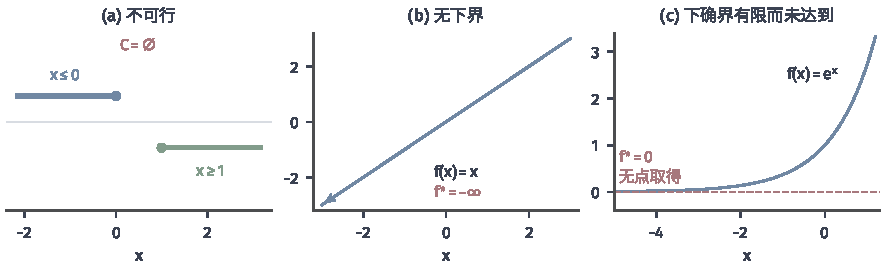
\includegraphics[width=150mm]{figures/03-optimization-evolution-and-signals/01-optimization/matplotlib/c1-failure-modes/figure.pdf}
  \caption{优化问题没有最优解的三种方式。(a) 约束$x\leq0$（蓝）与$x\geq1$（绿）没有公共点，可行域为空。(b) $f(x)=x$在实轴上沿箭头方向无限下降，最优值为$-\infty$。(c) $f(x)=e^x$的值趋于红色虚线$0$却永不等于$0$：最优值有限，但没有可行点取得它。}
  \label{fig:opt-prob-failure-modes}
\end{figure*}

到目前为止，我们假定目标在每个可行点上取有限实数值。第~\ref{sec:opt-prob-extended-value}小节将允许目标取$+\infty$，届时再检查这些定义是否仍然适用。

\subsection{局部最优与全局最优}
\label{sec:opt-prob-local-global}

站在地形中的一个洼地底部，向四周看处处都更高，但山那边可能还有更深的谷。只和附近比较，与和所有可行点比较，是两个不同的要求。下面用欧氏开球$B(\bm x,r)=\{\bm y:\lVert\bm y-\bm x\rVert_2<r\}$刻画“附近”。

\begin{definition}[局部最优与全局最优]
\label{def:opt-prob-local-global}
设$\bm x^\star\in C$。若$f(\bm x^\star)\leq f(\bm x)$对所有$\bm x\in C$成立，称$\bm x^\star$为\term{全局最优解}（global minimizer）。若存在$r>0$，使$f(\bm x^\star)\leq f(\bm x)$对所有$\bm x\in C\cap B(\bm x^\star,r)$成立，称$\bm x^\star$为\term{局部最优解}（local minimizer）；若进一步对所有$\bm x\in C\cap B(\bm x^\star,r)$、$\bm x\neq\bm x^\star$有严格不等式，称为\term{严格局部最优解}（strict local minimizer）。
\end{definition}

全局最优解就是定义~\ref{def:opt-prob-optimal-value}中的最优解。局部比较的范围是$C\cap B(\bm x^\star,r)$而不是整个球：可行域边界上的点只需与球内的可行点比较，球中伸出可行域的部分不参加比较。

\begin{example}[边界上的最优与多个洼地]
\label{ex:opt-prob-local-global}
取$f(x)=x^4/4-x^3/3-x^2$，可行域$C=[-1.5,1.5]$。导数$f'(x)=x^3-x^2-2x=x(x-2)(x+1)$在$x=-1,0,2$处为零。计算得$f(-1)=-5/12\approx-0.417$，$f(0)=0$，$f(1.5)\approx-2.109$，$f(-1.5)\approx0.141$。由$f'$的符号，$f$在$[-1.5,-1]$上递减、在$[-1,0]$上递增、在$[0,1.5]$上递减。所以$x=-1$附近的可行点函数值都不低于$-5/12$，它是局部最优解；而$C$上的最小值只能出现在$x=-1$或右端点$x=1.5$，后者更低，因此$x=1.5$是$C$上的全局最优解。在这个边界点处$f'(1.5)=-1.875\neq0$：函数仍在向右下降，只是可行域不允许再往右走。若去掉约束，最低点会移到$C$之外的$x=2$，$f(2)=-8/3$。
\end{example}

图~\ref{fig:opt-prob-local-global}画出这个例子。浅蓝色带是可行域，读者应注意三件事：$x=-1$是一个洼地底部，却不是最低处；全局最优落在可行域的边界上，那里的切线并不水平；可行域之外还有更低的点，它与问题无关。这说明局部最优与全局最优必须按定义区分，也说明不能先用“导数为零”代替最优解的定义——第~\ref{sec:opt-prob-optimality}节会看到，导数为零只在可行域内部的点上才是必要条件。

\begin{figure}[!htbp]
  \centering
  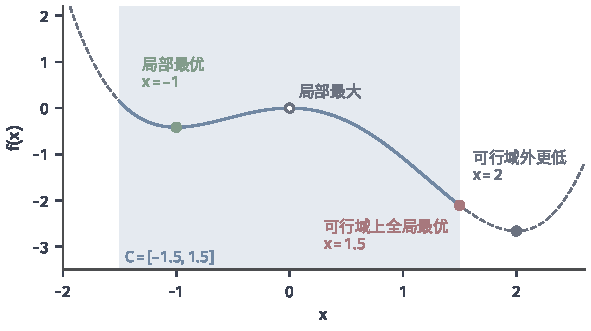
\includegraphics[width=100mm]{figures/03-optimization-evolution-and-signals/01-optimization/matplotlib/c1-local-global/figure.pdf}
  \caption{$f(x)=x^4/4-x^3/3-x^2$在可行域$C=[-1.5,1.5]$（浅蓝色带）上的局部与全局最优。蓝色实线是$C$上的图像，虚线是$C$外的部分。绿点$x=-1$是局部最优解，红点$x=1.5$是$C$上的全局最优解（该处导数为$-1.875$），空心点$x=0$是局部最大点，灰点$x=2$是$C$之外的更低点。}
  \label{fig:opt-prob-local-global}
\end{figure}

\paragraph{严格、唯一与多个等值解}
严格局部最优解在一个小邻域内是唯一的最低点，但这不排除远处还有同样低或更低的点。$f(x)=(x^2-1)^2$在$x=\pm1$处都取到全局最小值$0$，两点各自都是严格局部最优解，全局最优解却有两个。全局最优解唯一，是比“每个最优解都是严格局部最优”更强的整体性质。

\paragraph{参数不唯一而预测相同}
最小二乘实例在$\lambda=0$时给出一个更有实际意义的情形。此时$f(\bm x)=\tfrac12(x_1+x_2-2)^2\geq0$，凡满足$x_1+x_2=2$的点都使$f=0$，因而都是全局最优解；最优解集合是一整条直线（图~\ref{fig:opt-prob-ls-sublevel}(a)中的绿色虚线）。直线上任意两个参数，例如$(1,1)$与$(3,-1)$，对唯一的观测给出相同的预测$\bm A\bm x=2$。数据只约束了$x_1+x_2$，没有约束$x_1-x_2$；在给定样本上，选哪个参数都一样好，但若用它们去预测新的输入$(1,0)$，结果分别是$1$和$3$。参数不唯一不是计算的失败，而是问题本身没有提供区分它们的信息。

\subsection{扩展实值目标}
\label{sec:opt-prob-extended-value}

到目前为止，可行域和目标是两个分开的对象。后续章节常常要把几种代价相加，或者把约束子问题交给同一个工具处理，那时“$f$加上一个集合”很不方便。一个自然的想法是：让不可行的点取一个大到不可能被选中的值，从而不参加比较。取任何有限的大数都不够保险，于是允许取$+\infty$。

\begin{definition}[扩展实值函数、有效定义域与指示函数]
\label{def:opt-prob-extended}
取值于$\mathbb R\cup\{+\infty\}$的函数$f:\mathbb R^d\to\mathbb R\cup\{+\infty\}$称为\term{扩展实值函数}（extended real-valued function）。它的\term{有效定义域}（effective domain）是$\operatorname{dom}f=\{\bm x:f(\bm x)<+\infty\}$。若$\operatorname{dom}f\neq\varnothing$，称$f$为\term{适当函数}（proper function）。集合$C\subseteq\mathbb R^d$的\term{指示函数}（indicator function）为
\[
  \iota_C(\bm x)=\begin{cases}0,&\bm x\in C,\\+\infty,&\bm x\notin C.\end{cases}
\]
扩展实值目标的最优值仍为$f^\star=\inf_{\bm x\in\mathbb R^d}f(\bm x)$，最优解集合规定为$\argmin f=\{\bm x\in\operatorname{dom}f:f(\bm x)=f^\star\}$。
\end{definition}

这里不允许取$-\infty$，所以“适当”只需要求至少有一点取有限值。最优解集合只在有效定义域中寻找，这是为了排除一种错觉：若$f$处处为$+\infty$，则$f^\star=+\infty$，每一点都“等于最优值”，但没有一个点是可用的答案。

\paragraph{统一写法保留了什么}
给定非空$C$和$C$上的实值目标$f_0$，令$F(\bm x)=f_0(\bm x)$（$\bm x\in C$），$F(\bm x)=+\infty$（$\bm x\notin C$），也记作$F=f_0+\iota_C$。逐项核对：$\operatorname{dom}F=C$，所以$F$适当，有限值候选恰好是可行点；$F$与$f_0$在可行点上取值相同，在其余点取$+\infty$，不影响下确界，所以$\inf F=\inf_Cf_0$；最优解只在$\operatorname{dom}F=C$中找，因而$\argmin F=\argmin_Cf_0$。约束问题与它的扩展实值写法有相同的最优值和相同的最优解，“达到”与否也一致。若$C=\varnothing$，则$F\equiv+\infty$，不适当，应报告不可行，而不能说每一点都最优。

\paragraph{指示函数不同于惩罚}
要区分三种看起来相近的对象。指示函数$\iota_C$取$0$与$+\infty$，它把违规点彻底排除。取$0$与$1$的集合示性函数$\mathbb 1_C$（在$C$上为$1$、在$C$外为$0$）只是一个普通的有界函数，把它加到目标上不会禁止任何点。有限惩罚则给违规程度定价，例如在$C=\{x:x\leq1\}$上最小化$(x-2)^2$时，改用
\[
  (x-2)^2+\max\{0,x-1\}
\]
代替约束。当$x>1$时，该函数的导数$2(x-2)+1$在$x=1.5$处为零，此处函数值$0.25+0.5=0.75$小于可行最优值$(1-2)^2=1$，所以惩罚问题的最小点$x=1.5$违反了约束。图~\ref{fig:opt-prob-extended-value}画出了这一差别：惩罚只是“不喜欢”违规，指示函数才真正禁止违规。惩罚系数多大才能恢复约束、怎样逐步加大惩罚，是第~\ref{chap:constrained-optimization}章的话题。

\begin{figure}[!htbp]
  \centering
  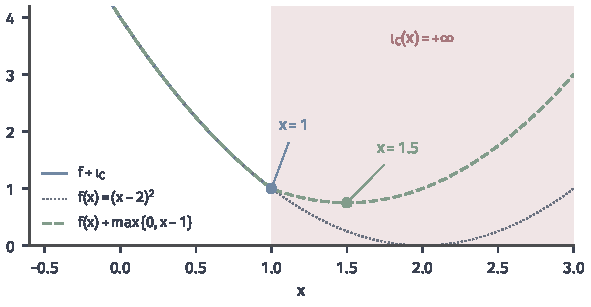
\includegraphics[width=100mm]{figures/03-optimization-evolution-and-signals/01-optimization/matplotlib/c1-extended-value/figure.pdf}
  \caption{指示函数与有限惩罚。目标$f(x)=(x-2)^2$（灰色点线），约束$x\leq1$。蓝线是$f+\iota_C$：在粉色区域$x>1$中取值$+\infty$，最小点为$x=1$、最小值为$1$。绿色虚线是加上惩罚$\max\{0,x-1\}$后的目标，最小点为$x=1.5$、最小值为$0.75$，落在约束之外。}
  \label{fig:opt-prob-extended-value}
\end{figure}

此后需要时，我们把约束问题~\eqref{eq:opt-prob-general}直接写成扩展实值目标的无约束最小化；两种写法描述同一个问题。

\section{最优解的存在}
\label{sec:opt-prob-existence}

上一节的$e^x$表明，最优值有限并不保证有点取得它。在讨论怎样求解之前，应当先确认所求的对象存在；否则一个算法“收敛”到的东西可能根本不是解。本节不构造任何算法，只问：一列越来越好的可行点，能否留下一个可行的极限，并把“好”传给这个极限。

\subsection{紧集与下半连续目标}
\label{sec:opt-prob-compact-lsc}

\paragraph{从最小化序列出发}
设$f^\star$有限。按下确界的定义，对每个$k$都有可行点$\bm x^{(k)}$满足$f(\bm x^{(k)})\leq f^\star+1/k$；若$f^\star=-\infty$，则改取$f(\bm x^{(k)})\leq-k$。这样的序列称为\term{最小化序列}（minimizing sequence），它的目标值趋于$f^\star$。这里的上标$(k)$只是序列编号，不表示任何算法的迭代。要从它得到最优解，需要依次完成三个环节：

\begin{enumerate}
  \item 序列有收敛的子列，即候选不会散开或逃向无穷远；
  \item 子列的极限仍然可行；
  \item 目标值的比较能传到极限，即极限处的目标值不高于序列目标值的极限。
\end{enumerate}

前两个环节由可行域负责，第三个环节由目标函数负责。在$\mathbb R^d$中，有界闭集的每个序列都有收敛子列，且极限仍在集合内，即有界闭集是紧集；这正好完成前两个环节（可参考\BookChapterRef{chap:metric-spaces}{卷二“度量空间”章}中紧致性的序列刻画与欧氏空间的闭有界判据）。第三个环节若用连续性完成，就得到熟悉的结论：有界闭集上的连续函数取得最小值，卷一已经在多元函数中建立（可参考\BookChapterRef{chap:multivariate-calculus}{卷一“多元函数微分”章}）。

\paragraph{只需要单向的比较}
仔细看第三个环节：我们只需要极限处的值“不比序列高”，不需要它“等于序列的极限”。函数可以在极限点向下跳，那只会让极限点更好；不能允许的是向上跳。这个单向条件就是下半连续性。

\begin{definition}[下半连续]
\label{def:opt-prob-lsc}
设$C\subseteq\mathbb R^d$，$f:C\to\mathbb R\cup\{+\infty\}$。若对$C$中每个收敛到$\bm x\in C$的序列$\bm x^{(k)}$，都有
\[
  f(\bm x)\leq\liminf_{k\to\infty}f(\bm x^{(k)}),
\]
就称$f$在$C$上\term{下半连续}（lower semicontinuous）。
\end{definition}

连续函数满足这个条件且取等号。下半连续还可以用“水平以下的部分”来刻画，这一刻画在下一小节是关键工具。对实数$a$，称$\{\bm x\in C:f(\bm x)\leq a\}$为$f$的\term{下水平集}（sublevel set），即地形图上高度不超过$a$的区域。

\begin{lemma}[下半连续与闭下水平集]
\label{lem:opt-prob-lsc-sublevel}
设$C\subseteq\mathbb R^d$闭，$f:C\to\mathbb R\cup\{+\infty\}$。$f$在$C$上下半连续，当且仅当对每个$a\in\mathbb R$，下水平集$\{\bm x\in C:f(\bm x)\leq a\}$是$\mathbb R^d$中的闭集。
\end{lemma}

\begin{proof}
设$f$下半连续，$\bm x^{(k)}$属于水平$a$的下水平集且收敛到$\bm x$。$C$闭，所以$\bm x\in C$；由下半连续，$f(\bm x)\leq\liminf_kf(\bm x^{(k)})\leq a$，极限仍在下水平集中，故下水平集闭。

反过来，设各下水平集都闭，但$f$在某点$\bm x\in C$不满足下半连续：存在$C$中的序列$\bm x^{(k)}\to\bm x$，使$\liminf_kf(\bm x^{(k)})<f(\bm x)$。取实数$a$介于二者之间，则有子列始终满足$f(\bm x^{(k_j)})\leq a$，即子列落在水平$a$的下水平集中；该集合闭，所以极限$\bm x$也在其中，$f(\bm x)\leq a$，与$a<f(\bm x)$矛盾。
\end{proof}

图~\ref{fig:opt-prob-lsc-gap}比较了两个只在跳跃点处取值不同的函数。左图在跳跃点取下方的值$0.4$，高度不超过$0.6$的点组成闭区间$[0,0.4]$；右图在跳跃点取上方的值$1$，同一个下水平集变成$(0,0.4]$，缺了左端点。右图的函数在$[-1,1.5]$上的下确界是$0.4$，沿$x\downarrow0$可以无限接近，却在$x=0$处被“跳高”挡住，没有点取得它。读者应从图中看到：下半连续性的作用，正是让下水平集不缺边界。

\begin{figure}[!htbp]
  \centering
  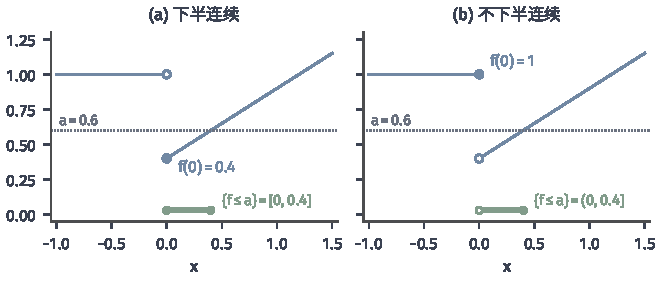
\includegraphics[width=112mm]{figures/03-optimization-evolution-and-signals/01-optimization/matplotlib/c1-lsc-gap/figure.pdf}
  \caption{下半连续与下水平集的缺口。两个函数在$x<0$时都等于$1$，在$x>0$时都等于$0.4+0.5x$，只在$x=0$处取值不同（实心点）。灰色点线是水平$a=0.6$，绿色线段是下水平集$\{f\leq0.6\}$。(a) $f(0)=0.4$，函数下半连续，下水平集为闭区间$[0,0.4]$；(b) $f(0)=1$，在$0$处向上跳，不下半连续，下水平集$(0,0.4]$缺少端点。}
  \label{fig:opt-prob-lsc-gap}
\end{figure}

\paragraph{紧可行域上的存在定理}
三个环节齐备，就得到存在性。

\begin{theorem}[紧可行域上的最小值]
\label{thm:opt-prob-compact-existence}
设$C\subseteq\mathbb R^d$非空且紧，$f:C\to\mathbb R\cup\{+\infty\}$在$C$上下半连续，且至少有一点$\bm x\in C$使$f(\bm x)<+\infty$。则$f^\star=\inf_{\bm x\in C}f(\bm x)$是有限实数，且最优解集合非空。
\end{theorem}

\begin{proof}
由假设$f^\star<+\infty$。取最小化序列$\bm x^{(k)}\in C$：$f^\star$有限时要求$f(\bm x^{(k)})\leq f^\star+1/k$，$f^\star=-\infty$时要求$f(\bm x^{(k)})\leq-k$。$C$紧，故有子列$\bm x^{(k_j)}\to\bm x^\star\in C$。由下半连续，
\[
  f(\bm x^\star)\leq\liminf_{j\to\infty}f(\bm x^{(k_j)})=f^\star.
\]
若$f^\star=-\infty$，上式给出$f(\bm x^\star)=-\infty$，与$f$不取$-\infty$矛盾，所以$f^\star$有限。又$\bm x^\star$可行，$f(\bm x^\star)\geq f^\star$；两个不等式合起来得$f(\bm x^\star)=f^\star$，$\bm x^\star$是最优解。
\end{proof}

资源分配的可行域是四条闭半平面的交，有界且闭，目标是线性函数，因而连续；定理~\ref{thm:opt-prob-compact-existence}立即保证最优解存在。这个结论不需要知道最优解在$(2,2)$，它只确认值得去找。

\paragraph{三个环节各自的失效}
图~\ref{fig:opt-prob-existence-failures}用三个例子分别拆掉一个环节。(a) 在$C=(0,1]$上最小化$f(x)=x$：最小化序列$2^{-k}$收敛到$0$，但$0$不在$C$中，失败在“极限可行”；$C$有界但不闭。(b) 在$C=[1,\infty)$上最小化$f(x)=1/x$：$C$闭但无界，序列$2^k$的目标值趋于下确界$0$，自身却逃向无穷远，没有收敛子列，失败在“序列留在有界区域”。(c) 在紧集$C=[-1,1]$上，令$f(x)=x^2$（$x\neq0$）、$f(0)=0.6$：序列$1/k$收敛到$0$，目标值趋于$0$，但极限处函数值跳到$0.6$，下确界$0$未被达到，失败在“比较传到极限”，因为$f$在$0$处不下半连续。三个条件缺一不可，但它们都只是充分条件：例如$f(x)=x^2$在无界的$\mathbb R$上仍有最小点。

\begin{figure*}[!htbp]
  \centering
  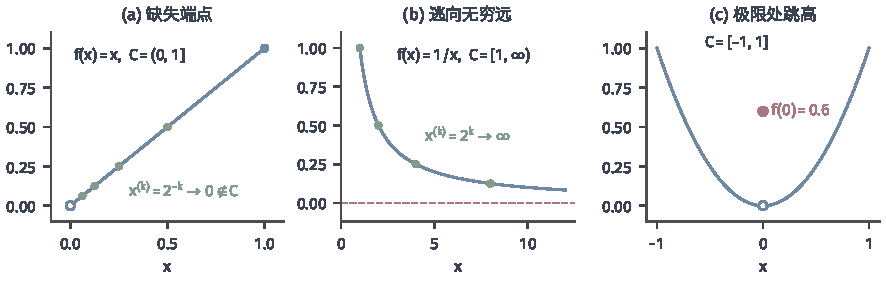
\includegraphics[width=150mm]{figures/03-optimization-evolution-and-signals/01-optimization/matplotlib/c1-existence-failures/figure.pdf}
  \caption{存在性论证的三个环节分别失效。绿点是最小化序列。(a) $f(x)=x$，$C=(0,1]$：序列$2^{-k}$趋于不可行的端点$0$（空心点）。(b) $f(x)=1/x$，$C=[1,\infty)$：序列$2^k$逃向无穷远，目标值趋于红色虚线$0$。(c) $f(x)=x^2$（$x\neq0$），$f(0)=0.6$，$C=[-1,1]$：序列趋于$0$时目标值趋于$0$，但$f(0)$跳高到$0.6$（红点），空心点处的值$0$无人取得。}
  \label{fig:opt-prob-existence-failures}
\end{figure*}

\subsection{强制性与紧下水平集}
\label{sec:opt-prob-coercive}

\paragraph{无界可行域怎么办}
最小二乘的可行域是整个$\mathbb R^d$，它不紧，定理~\ref{thm:opt-prob-compact-existence}不能直接用。但我们并不需要整个可行域紧，只需要最小化序列被关在某个紧集里。取一个可行点$\bar{\bm x}$，凡是目标值比$f(\bar{\bm x})$还高的点都不可能是最优解，可以直接丢掉；剩下的是下水平集$\{\bm x\in C:f(\bm x)\leq f(\bar{\bm x})\}$。如果这个集合紧，问题就回到紧集上。它闭的条件已由引理~\ref{lem:opt-prob-lsc-sublevel}给出，还缺有界：目标必须在远处足够高，使“不太差的点”不会跑到无穷远。

\begin{definition}[强制性]
\label{def:opt-prob-coercive}
设$C\subseteq\mathbb R^d$，$f:C\to\mathbb R\cup\{+\infty\}$。若对$C$中任意满足$\lVert\bm x^{(k)}\rVert_2\to\infty$的序列都有$f(\bm x^{(k)})\to+\infty$，就称$f$在$C$上是\term{强制的}（coercive）。$C$有界时，这个条件自动成立。
\end{definition}

强制性等价于：每个下水平集都有界。若某个水平$a$的下水平集无界，从中取范数趋于无穷的序列，其目标值始终不超过$a$，与强制性矛盾；反过来，若各下水平集都有界，而$\lVert\bm x^{(k)}\rVert_2\to\infty$，则对任意$a$，序列最终离开水平$a$的下水平集，即最终$f(\bm x^{(k)})>a$，所以$f(\bm x^{(k)})\to+\infty$。

\begin{theorem}[强制目标的最小值]
\label{thm:opt-prob-coercive-existence}
设$C\subseteq\mathbb R^d$非空且闭，$f:C\to\mathbb R\cup\{+\infty\}$在$C$上下半连续且强制，并且存在$\bar{\bm x}\in C$使$f(\bar{\bm x})<+\infty$。则$f^\star$是有限实数，且最优解集合非空。
\end{theorem}

\begin{proof}
令$K=\{\bm x\in C:f(\bm x)\leq f(\bar{\bm x})\}$。它含有$\bar{\bm x}$，非空；由引理~\ref{lem:opt-prob-lsc-sublevel}，它是闭集；由强制性，它有界。于是$K$紧，$f$限制在$K$上仍下半连续，定理~\ref{thm:opt-prob-compact-existence}给出$\bm x^\star\in K$，使$f(\bm x^\star)=\min_Kf\leq f(\bar{\bm x})$。对$C\setminus K$中的点，$f(\bm x)>f(\bar{\bm x})\geq f(\bm x^\star)$。所以$\bm x^\star$是$f$在整个$C$上的最小点，$f^\star=f(\bm x^\star)$有限。
\end{proof}

证明中各条件的分工很清楚：强制性让下水平集有界，留住了序列；$C$闭与下半连续让下水平集闭，留住了极限；剩下的工作交给紧集上的定理。

\paragraph{回到最小二乘}
对式~\eqref{eq:opt-prob-ridge}逐项核对。$f$是多项式，处处有限，因而适当且连续；$C=\mathbb R^d$闭，加上非负约束后$C=\{\bm x:\bm x\geq\bm 0\}$也是闭集。当$\lambda>0$时，$f(\bm x)\geq\frac{\lambda}{2}\lVert\bm x\rVert_2^2$，范数趋于无穷时目标趋于无穷，$f$强制。由定理~\ref{thm:opt-prob-coercive-existence}，无论是否加非负约束，最优解都存在。

$\lambda=0$时情况不同。在最小二乘实例中，$f(\bm x)=\frac12(x_1+x_2-2)^2$沿方向$(1,-1)$保持不变：取$\bm x^{(k)}=(1+k,1-k)$，范数趋于无穷而$f=0$，所以$f$不强制，水平$1$的下水平集是一条无界的带。图~\ref{fig:opt-prob-ls-sublevel}比较了两种情形：$\lambda=0.5$时同一水平的下水平集收缩为一个椭圆，$\lambda=0$时则沿最优解直线无限延伸。然而$\lambda=0$时最优解仍然存在——整条直线$x_1+x_2=2$都是。这说明强制性只是充分条件；对一般的$\bm A$，无正则最小二乘总有解，这由正规方程的可解性保证，而不是由强制性保证（可参考\BookChapterRef{chap:linear-equations-and-optimization}{卷一“线性方程与矩阵方程”章}）。若$\bm A$列满秩，则对$\bm x\neq\bm 0$有$\bm A\bm x\neq\bm 0$，在单位球面上取最小值可得常数$\sigma>0$使$\lVert\bm A\bm x\rVert_2\geq\sigma\lVert\bm x\rVert_2$，此时即使$\lambda=0$，$f$也强制。

\begin{figure*}[!htbp]
  \centering
  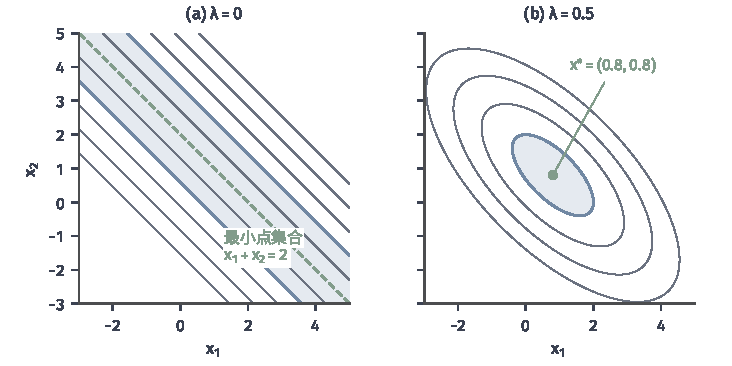
\includegraphics[width=124mm]{figures/03-optimization-evolution-and-signals/01-optimization/matplotlib/c1-ls-sublevel/figure.pdf}
  \caption{最小二乘实例$f(\bm x)=\frac12(x_1+x_2-2)^2+\frac{\lambda}{2}\lVert\bm x\rVert_2^2$的下水平集。浅蓝区域及其蓝色边界是$\{f\leq1\}$，灰线是$f=0.25,2.25,4,6.25$的等值线。(a) $\lambda=0$：下水平集是两条平行线之间的无界带，最优解集合是绿色虚线$x_1+x_2=2$。(b) $\lambda=0.5$：下水平集是有界椭圆，唯一最优解为$\bm x^\star=(0.8,0.8)$，最优值为$0.4$。}
  \label{fig:opt-prob-ls-sublevel}
\end{figure*}

\paragraph{有限维的边界}
整个论证依赖“有界闭集紧”这一有限维性质。在无限维空间中它不成立：例如平方可和序列空间中，第$k$个坐标为$1$、其余为$0$的单位向量$\bm e_k$两两距离都是$\sqrt2$，它们都在闭单位球中，却没有收敛子列。于是即使目标强制、下水平集有界闭，最小化序列也可能没有极限。处理函数空间中的存在性需要更弱的收敛概念，这是第~\ref{chap:opt-functional}章的任务。

\section{凸性与解的性质}
\label{sec:opt-prob-convexity}

存在性只回答“有没有”。站在一个洼地底部时，我们还想知道：山那边会不会有更深的谷？最低点是不是只有一个？离最低点还有多远？这些问题都涉及两个候选之间的比较，而最简单的比较路径是连接它们的线段。本节先要求线段留在可行域内（凸集），再要求目标沿线段不高于端点的加权平均（凸函数），然后逐步加强这一要求：严格凸排除多个最小点，强凸再给出统一的二次间隔，把目标差换算成到最小点的距离。

\subsection{凸集与凸组合}
\label{sec:opt-prob-convex-sets}

资源分配中，若方案$P=(3,0)$与$Q=(0,4)$都可行，各按一半执行的混合方案$M=\frac12P+\frac12Q=(1.5,2)$也可行：$1.5+2=3.5\leq4$，$3+2=5\leq6$。这不是巧合，因为线性约束在混合下保持：若$\langle\bm g,\bm u\rangle\leq h$且$\langle\bm g,\bm v\rangle\leq h$，则对$\theta\in[0,1]$，$\langle\bm g,\theta\bm u+(1-\theta)\bm v\rangle\leq\theta h+(1-\theta)h=h$。可行方案任意混合仍可行，正是凸集的定义。

\begin{definition}[凸集与凸组合]
\label{def:opt-prob-convex-set}
若对任意$\bm u,\bm v\in C$与$\theta\in[0,1]$都有$\theta\bm u+(1-\theta)\bm v\in C$，称$C\subseteq\mathbb R^d$为\term{凸集}（convex set）。对点$\bm a_1,\dots,\bm a_k$，若$\alpha_i\geq0$且$\sum_{i=1}^k\alpha_i=1$，称$\sum_{i=1}^k\alpha_i\bm a_i$为它们的一个\term{凸组合}（convex combination）。集合$A$中点的全部有限凸组合组成的集合称为$A$的\term{凸包}（convex hull），记作$\operatorname{conv}A$。
\end{definition}

几何上，凸集里任意两点之间的线段都留在集合内。图~\ref{fig:opt-prob-convex-sets}给出对照：椭圆盘中的线段始终在盘内；月牙形中，上下两个尖端附近的点都在集合里，连接它们的线段却穿过缺口；资源分配的四边形里，两个可行方案的混合点$M$落在连接它们的线段上，仍然可行。

\begin{figure}[!htbp]
  \centering
  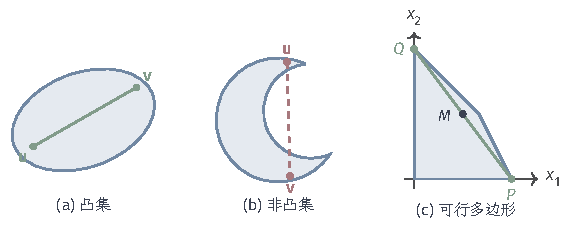
\includegraphics[width=97.017mm]{figures/03-optimization-evolution-and-signals/01-optimization/tikz/c1-convex-sets/figure.pdf}
  \caption{凸集与非凸集。(a) 椭圆盘：任意两点$\bm u,\bm v$之间的线段（绿色）留在集合内。(b) 月牙形：两点都在集合中，连接它们的红色虚线却穿过缺口，所以不是凸集。(c) 资源分配的可行四边形：方案$P=(3,0)$与$Q=(0,4)$的等权混合$M=(1.5,2)$仍在四边形内。}
  \label{fig:opt-prob-convex-sets}
\end{figure}

\paragraph{常见的凸集}
以下几类集合在后文反复出现。对非零$\bm g\in\mathbb R^d$与$h\in\mathbb R$，\term{半空间}（halfspace）$\{\bm x:\langle\bm g,\bm x\rangle\leq h\}$是凸集，上面的计算就是证明。有限个半空间的交称为\term{多面体}（polyhedron），资源分配的可行域$\{\bm x:\bm G\bm x\leq\bm h,\ \bm x\geq\bm 0\}$就是一个多面体，它是第~\ref{chap:opt-linear-programming}章的主角。闭球$\{\bm x:\lVert\bm x-\bm a\rVert_2\leq r\}$是凸集：由三角不等式，$\lVert\theta\bm u+(1-\theta)\bm v-\bm a\rVert_2\leq\theta\lVert\bm u-\bm a\rVert_2+(1-\theta)\lVert\bm v-\bm a\rVert_2\leq r$，对任何范数的球都成立。$d\times d$对称半正定矩阵组成的集合也是凸集：对每个固定的$\bm v$，条件$\bm v^\top\bm X\bm v\geq0$是关于矩阵$\bm X$的线性不等式，半正定矩阵集合是所有这些条件的交。第~\ref{chap:constrained-optimization}章的矩阵约束将用到它。

\paragraph{保持凸性的运算}
判断一个集合是否凸，通常不直接验证定义，而是把它拆成已知凸集经过保凸运算得到的结果。设$\bm M\in\mathbb R^{k\times d}$，$\bm q\in\mathbb R^k$。
\begin{itemize}
  \item 任意多个凸集的交是凸集：两点都在每个集合中，线段也在每个集合中。
  \item 凸集$C\subseteq\mathbb R^d$在仿射映射下的像$\{\bm M\bm x+\bm q:\bm x\in C\}$是凸集：像点的凸组合$\theta(\bm M\bm u+\bm q)+(1-\theta)(\bm M\bm v+\bm q)=\bm M(\theta\bm u+(1-\theta)\bm v)+\bm q$仍是像点。
  \item 凸集$D\subseteq\mathbb R^k$的仿射逆像$\{\bm x:\bm M\bm x+\bm q\in D\}$是凸集：用同一个等式反向读即可。
\end{itemize}
半空间是一维区间$(-\infty,h]$在线性映射$\bm x\mapsto\langle\bm g,\bm x\rangle$下的逆像，多面体是半空间的交，这两条规则就足以确认资源分配可行域是凸集。

\paragraph{凸包与闭凸包}
二点线段可以反复使用。若$C$凸，对点数归纳可知$C$包含其中任意有限个点的凸组合：$k$个点的凸组合在$\alpha_k<1$时可以写成
\[
  \sum_{i=1}^k\alpha_i\bm a_i=(1-\alpha_k)\sum_{i=1}^{k-1}\frac{\alpha_i}{1-\alpha_k}\bm a_i+\alpha_k\bm a_k,
\]
括号里的系数非负且和为$1$，是$k-1$个点的凸组合，再与$\bm a_k$作二点组合；$\alpha_k=1$时组合就是$\bm a_k$本身。另一方面，两个凸组合的凸组合展开后仍是凸组合，所以$\operatorname{conv}A$自身是凸集。二者合起来说明：$\operatorname{conv}A$是包含$A$的最小凸集。资源分配的四边形恰好是它四个顶点的凸包，有界多面体与其顶点的这一关系将在第~\ref{chap:opt-linear-programming}章建立。

凸包不一定是闭集，即使$A$本身闭。取$A=\{(0,0)\}\cup\{(t,1):t\in\mathbb R\}$，它是一个点与一条直线的并，是闭集。原点与直线上的点$(x/y,1)$按权重$1-y$与$y$组合得到$(x,y)$，所以$0<y\leq1$的点都在$\operatorname{conv}A$中；而所有组合的第二个坐标都是权重的平均，非负且只有全部权重给原点时才为零，所以$y=0$的点中只有原点可达。于是$\operatorname{conv}A=\{(0,0)\}\cup\{(x,y):0<y\leq1\}$不闭，它的闭包是带$\{(x,y):0\leq y\leq1\}$。包含$A$的最小闭凸集称为\term{闭凸包}（closed convex hull），它等于$\operatorname{conv}A$的闭包。在需要取极限的论证中，应当用闭凸包而不是凸包；本章只用到这两个对象的定义，一般凸集的分离性质留到后续需要时建立。

\subsection{凸函数与一阶支撑}
\label{sec:opt-prob-convex-functions}

有了凸的可行域，两个可行点之间的线段上都是可行点。接下来要求目标沿这条线段“不鼓起来”：线段上每一点的目标值，不超过两端目标值按相同权重的平均。

\begin{definition}[凸函数]
\label{def:opt-prob-convex-function}
设$C\subseteq\mathbb R^d$为凸集。若函数$f:C\to\mathbb R$对任意$\bm u,\bm v\in C$与$\theta\in[0,1]$满足
\begin{equation}
  f\bigl(\theta\bm u+(1-\theta)\bm v\bigr)\leq\theta f(\bm u)+(1-\theta)f(\bm v),
  \label{eq:opt-prob-convex-function}
\end{equation}
称$f$为$C$上的\term{凸函数}（convex function）。扩展实值函数$f:\mathbb R^d\to\mathbb R\cup\{+\infty\}$称为凸函数，是指$\operatorname{dom}f$为凸集，且式~\eqref{eq:opt-prob-convex-function}对$\operatorname{dom}f$中的点成立。若$-f$凸，称$f$凹。
\end{definition}

式~\eqref{eq:opt-prob-convex-function}的右端是连接$(\bm u,f(\bm u))$与$(\bm v,f(\bm v))$的弦上的点，左端是同一位置的函数值，所以凸函数的图像位于每条弦的下方。图~\ref{fig:opt-prob-chord-tangent}(a)画出了$f(x)=x^2/2$及连接$x=-1$与$x=2$的弦。扩展实值情形只在有效定义域内检验，这避免了$0\cdot(+\infty)$之类无意义的运算；对$F=f_0+\iota_C$，它恰好要求$C$凸且$f_0$在$C$上凸。

\paragraph{上图与Jensen不等式}
另一种看法是把函数图像以上的区域当作一个集合。$f$的\term{上图}（epigraph）是$\operatorname{epi}f=\{(\bm x,s)\in\mathbb R^d\times\mathbb R:\bm x\in\operatorname{dom}f,\ f(\bm x)\leq s\}$。$f$凸当且仅当$\operatorname{epi}f$是凸集。若$f$凸，$(\bm u,s),(\bm v,t)$在上图中，则$f(\theta\bm u+(1-\theta)\bm v)\leq\theta f(\bm u)+(1-\theta)f(\bm v)\leq\theta s+(1-\theta)t$，混合点仍在上图中；反过来，取$s=f(\bm u)$、$t=f(\bm v)$，上图凸就给出式~\eqref{eq:opt-prob-convex-function}。凸函数与凸集因此是同一几何概念的两种说法。

把二点不等式按上一小节的方式对点数归纳，得到有限形式的\term{Jensen不等式}（Jensen's inequality）：对凸函数$f$、$\operatorname{dom}f$中的点$\bm x_1,\dots,\bm x_k$与凸组合系数$\alpha_i$，
\[
  f\Bigl(\sum_{i=1}^k\alpha_i\bm x_i\Bigr)\leq\sum_{i=1}^k\alpha_if(\bm x_i).
\]
系数必须非负且和为$1$：允许负系数时，组合点可以落到这些点的凸包之外，不等式不再有保证。

\paragraph{保凸规则}
与凸集一样，凸函数通常由简单的凸函数拼出来。直接由定义可以验证：凸函数的非负加权和是凸函数；凸函数与仿射映射的复合$\bm x\mapsto f(\bm M\bm x+\bm q)$是凸函数，因为仿射映射把线段映成线段。以最小二乘为例，先验证$\frac12\lVert\cdot\rVert_2^2$凸：展开内积可得恒等式
\begin{equation}
  \theta\lVert\bm u\rVert_2^2+(1-\theta)\lVert\bm v\rVert_2^2-\lVert\theta\bm u+(1-\theta)\bm v\rVert_2^2=\theta(1-\theta)\lVert\bm u-\bm v\rVert_2^2\geq0.
  \label{eq:opt-prob-square-identity}
\end{equation}
于是$\frac12\lVert\bm A\bm x-\bm b\rVert_2^2$是它与仿射映射$\bm x\mapsto\bm A\bm x-\bm b$的复合，$\frac{\lambda}{2}\lVert\bm x\rVert_2^2$是它的非负倍数，二者之和即式~\eqref{eq:opt-prob-ridge}是凸函数。资源分配的目标是线性函数，式~\eqref{eq:opt-prob-convex-function}取等号，既凸又凹。

一般的非线性复合则需要额外条件。$h(u)=u^2$与$k(x)=x^2-1$都是凸函数，复合$h(k(x))=(x^2-1)^2$却不凸：$x=\pm1$处函数值为$0$，中点$x=0$处为$1$，高于弦。一个常用的充分条件是：$k$凸，$h$凸且单调不减。此时$k(\theta u+(1-\theta)v)\leq\theta k(u)+(1-\theta)k(v)$，$h$不减保持这个不等式，再用$h$的凸性即得$h\circ k$凸。上例中$h(u)=u^2$在$u<0$时递减，不满足这一条件。

\paragraph{一阶支撑下界}
凸函数的图像在弦的下方；若函数可微，它还在每一点切线（切平面）的上方。图~\ref{fig:opt-prob-chord-tangent}把两者画在一起：左图凸函数的切线处处位于图像下方，右图非凸函数在$x=0$处的水平切线却位于图像上方的一大段区域。切线来自单点的导数，若它是全局下界，单点信息就能告诉我们远处的函数值至少有多大。这正是凸性在优化中最有用的形式。

\begin{figure}[!htbp]
  \centering
  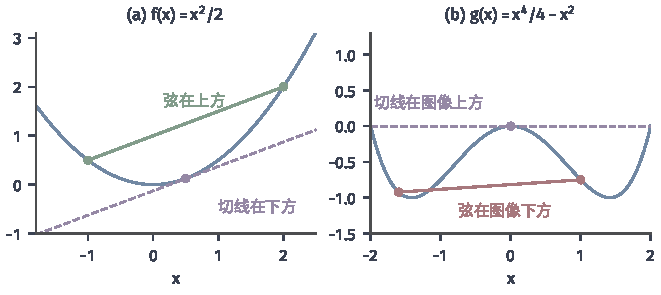
\includegraphics[width=112mm]{figures/03-optimization-evolution-and-signals/01-optimization/matplotlib/c1-chord-tangent/figure.pdf}
  \caption{弦与切线。(a) 凸函数$f(x)=x^2/2$：连接$x=-1$与$x=2$的绿色弦在两点之间位于图像上方，$x_0=1/2$处的紫色切线在整条实轴上位于图像下方。(b) 非凸函数$g(x)=x^4/4-x^2$：连接$x=-1.6$与$x=1$的红色弦有一段位于图像下方，$x=0$处的水平切线在$0<|x|<2$时位于图像上方，不再是下界。}
  \label{fig:opt-prob-chord-tangent}
\end{figure}

\begin{theorem}[凸性的一阶与二阶判据]
\label{thm:opt-prob-convex-criteria}
设$D\subseteq\mathbb R^d$是开凸集，$f:D\to\mathbb R$可微。
\begin{enumerate}
  \item $f$凸，当且仅当对任意$\bm u,\bm v\in D$，
  \begin{equation}
    f(\bm v)\geq f(\bm u)+\langle\nabla f(\bm u),\bm v-\bm u\rangle.
    \label{eq:opt-prob-first-order-support}
  \end{equation}
  \item 若$f$在$D$上二阶可微，则$f$凸当且仅当$\nabla^2f(\bm x)$对每个$\bm x\in D$半正定。
\end{enumerate}
\end{theorem}

\begin{proof}
(1) 设$f$凸。对$t\in(0,1]$，由式~\eqref{eq:opt-prob-convex-function}，$f(\bm u+t(\bm v-\bm u))\leq(1-t)f(\bm u)+tf(\bm v)$，整理得
\[
  \frac{f(\bm u+t(\bm v-\bm u))-f(\bm u)}{t}\leq f(\bm v)-f(\bm u).
\]
令$t\downarrow0$，左端趋于方向导数$\langle\nabla f(\bm u),\bm v-\bm u\rangle$，即得式~\eqref{eq:opt-prob-first-order-support}。反过来，设式~\eqref{eq:opt-prob-first-order-support}对所有点成立。取$\bm z=\theta\bm u+(1-\theta)\bm v$，分别以$\bm z$为切点、$\bm u$与$\bm v$为另一点：
\[
  f(\bm u)\geq f(\bm z)+\langle\nabla f(\bm z),\bm u-\bm z\rangle,\qquad
  f(\bm v)\geq f(\bm z)+\langle\nabla f(\bm z),\bm v-\bm z\rangle.
\]
第一式乘$\theta$、第二式乘$1-\theta$后相加，由$\theta(\bm u-\bm z)+(1-\theta)(\bm v-\bm z)=\bm 0$，内积项抵消，得到式~\eqref{eq:opt-prob-convex-function}。

(2) 设$f$凸，$\bm x\in D$，$\bm h\in\mathbb R^d$。$D$开，$t$充分小时$\bm x+t\bm h\in D$，由式~\eqref{eq:opt-prob-first-order-support}与二阶Taylor展开，
\[
  0\leq f(\bm x+t\bm h)-f(\bm x)-t\langle\nabla f(\bm x),\bm h\rangle=\frac{t^2}{2}\bm h^\top\nabla^2f(\bm x)\bm h+o(t^2).
\]
两端除以$t^2$再令$t\to0$，得$\bm h^\top\nabla^2f(\bm x)\bm h\geq0$。反过来，设Hessian处处半正定。对$\bm u,\bm v\in D$，令$\phi(t)=f(\bm u+t(\bm v-\bm u))$，$t\in[0,1]$，则$\phi''(t)=(\bm v-\bm u)^\top\nabla^2f(\bm u+t(\bm v-\bm u))(\bm v-\bm u)\geq0$，$\phi'$单调不减。一元函数导数单调不减时函数凸（由中值定理可得），所以$\phi(\theta\cdot0+(1-\theta)\cdot1)\leq\theta\phi(0)+(1-\theta)\phi(1)$，这正是式~\eqref{eq:opt-prob-convex-function}。
\end{proof}

定理中的Taylor展开与Hessian的计算见卷一；这里要强调的是两个判据的适用范围。它们都要求在整个开凸集上成立：在单个点检查Hessian半正定，不能证明函数凸。示例~\ref{ex:opt-prob-local-global}中的$f(x)=x^4/4-x^3/3-x^2$满足$f''(2)=6>0$，但$f''(0)=-2<0$，所以$f$不凸，也正因为不凸，它才会有不是全局最优的局部最优。对最小二乘，$\nabla^2f=\bm A^\top\bm A+\lambda\bm I$，对任意$\bm h$有$\bm h^\top(\bm A^\top\bm A+\lambda\bm I)\bm h=\lVert\bm A\bm h\rVert_2^2+\lambda\lVert\bm h\rVert_2^2\geq0$，与前面用保凸规则得到的结论一致。

\paragraph{局部最优即全局最优}
现在可以回答“山那边会不会有更深的谷”。

\begin{theorem}[凸问题的局部最优是全局最优]
\label{thm:opt-prob-local-global}
设$C$为凸集，$f:C\to\mathbb R$为凸函数。则$f$在$C$上的每个局部最优解都是全局最优解，并且最优解集合是凸集。
\end{theorem}

\begin{proof}
设$\bm u$是局部最优解，邻域半径为$r$。若存在$\bm v\in C$使$f(\bm v)<f(\bm u)$，对$t\in(0,1)$，点$\bm u+t(\bm v-\bm u)$在$C$中，且
\[
  f(\bm u+t(\bm v-\bm u))\leq(1-t)f(\bm u)+tf(\bm v)<f(\bm u).
\]
取$t$足够小，使$t\lVert\bm v-\bm u\rVert_2<r$，这个更低的点落在$C\cap B(\bm u,r)$中，与局部最优矛盾。所以$\bm u$是全局最优解。若$\bm u,\bm v$都是最优解，线段上的点满足$f\leq\theta f^\star+(1-\theta)f^\star=f^\star$，也是最优解，故最优解集合凸。
\end{proof}

证明的几何意义是：如果远处有更低的点，连向它的线段会从当前点出发立即下降，“假谷底”不可能存在。证明没有用到可微性，对非光滑的凸目标同样成立。最小二乘实例在$\lambda=0$时的最优解集合是一条直线，与定理的“最优解集合凸”一致。凸集与凸函数的系统处理可参考Boyd与Vandenberghe的教材\scite{math-boyd2004convex}。

\subsection{严格凸性与唯一性}
\label{sec:opt-prob-strict-convexity}

凸性排除了“假谷底”，但没有排除平坦的谷底：$\lambda=0$的最小二乘实例沿直线$x_1+x_2=2$处处最优。要让最优解唯一，需要线段上的不等式在两端不同时严格成立。

\begin{definition}[严格凸函数]
\label{def:opt-prob-strict-convex}
设$C$为凸集，$f:C\to\mathbb R$。若对任意$\bm u\neq\bm v$与$\theta\in(0,1)$，式~\eqref{eq:opt-prob-convex-function}严格成立，称$f$为\term{严格凸}（strictly convex）函数。
\end{definition}

\begin{theorem}[严格凸目标至多有一个最小点]
\label{thm:opt-prob-strict-unique}
设$C$为凸集，$f$在$C$上严格凸，则$\argmin_{\bm x\in C}f$至多含一个点。若再有最优解存在，则最优解唯一。
\end{theorem}

\begin{proof}
若$\bm u\neq\bm v$都是最优解，则中点$\frac12(\bm u+\bm v)\in C$满足$f(\frac12(\bm u+\bm v))<\frac12f^\star+\frac12f^\star=f^\star$，与$f^\star$是下确界矛盾。
\end{proof}

定理的结论是“至多一个”，存在性必须另外由上一节的条件保证。正反两个方向都有反例。$e^x$在$\mathbb R$上严格凸（二阶导数处处为正），却没有最小点：严格凸不推出存在。$|x|$有唯一最小点$0$，但在$[0,1]$上是线性的，式~\eqref{eq:opt-prob-convex-function}取等号，不严格凸：最小点唯一不推出严格凸。资源分配是一个更实际的例子：线性目标处处不严格凸，最优解$(2,2)$却是唯一的，唯一性来自可行域的顶点，而不是目标的弯曲。

\paragraph{二次函数的一个恒等式}
最小二乘是二次函数，严格凸可以直接读出来。设$q(\bm x)=\frac12\bm x^\top\bm H\bm x+\bm g^\top\bm x+c$，$\bm H$对称。仿照式~\eqref{eq:opt-prob-square-identity}展开，线性项与常数项在加权平均中抵消，得到
\begin{equation}
  \theta q(\bm u)+(1-\theta)q(\bm v)-q\bigl(\theta\bm u+(1-\theta)\bm v\bigr)=\frac12\theta(1-\theta)(\bm u-\bm v)^\top\bm H(\bm u-\bm v).
  \label{eq:opt-prob-quadratic-identity}
\end{equation}
左端是弦与函数之间的间隔，它完全由$\bm H$在方向$\bm u-\bm v$上的二次型决定。于是$q$凸当且仅当$\bm H$半正定，严格凸当且仅当$\bm H$正定：若$\bm H$半正定但奇异，取零空间中的非零方向$\bm w$，沿该方向的线段上间隔为零，不严格凸。

最小二乘目标展开为$f(\bm x)=\frac12\bm x^\top(\bm A^\top\bm A+\lambda\bm I)\bm x-\bm b^\top\bm A\bm x+\frac12\lVert\bm b\rVert_2^2$，$\bm H=\bm A^\top\bm A+\lambda\bm I$。对非零$\bm w$，$\bm w^\top\bm H\bm w=\lVert\bm A\bm w\rVert_2^2+\lambda\lVert\bm w\rVert_2^2$。$\lambda>0$时它为正；$\lambda=0$时它为正当且仅当$\bm A\bm w\neq\bm 0$对所有非零$\bm w$成立，即$\bm A$列满秩。所以$\lambda>0$或$\bm A$列满秩时目标严格凸，再结合上一节的存在性，最优解唯一。在最小二乘实例中，$\bm H=\begin{pmatrix}1+\lambda&1\\1&1+\lambda\end{pmatrix}$；$\lambda=0$时$\bm w=(1,-1)$使$\bm w^\top\bm H\bm w=0$，最优解成线；$\lambda>0$时最优条件$(\bm A^\top\bm A+\lambda\bm I)\bm x=\bm A^\top\bm b=(2,2)^\top$有唯一解$\bm x^\star=\frac{2}{2+\lambda}(1,1)$，$\lambda=0.5$时即图~\ref{fig:opt-prob-ls-sublevel}(b)中的$(0.8,0.8)$。

\subsection{强凸性与误差控制}
\label{sec:opt-prob-strong-convexity}

严格凸只说弦与函数之间有间隔，没说间隔有多大。$x^4$严格凸，但在原点附近极其平坦：取$\bm u=-t$、$\bm v=t$、$\theta=\frac12$，间隔只有$\frac12t^4+\frac12t^4-0=t^4$，比两点距离的平方$4t^2$小得多。若间隔太小，目标值几乎相同的两个点可能相距很远，我们就无法从“目标值差不多最优”推断“参数差不多正确”。强凸性要求间隔至少与距离的平方成比例。

\begin{definition}[强凸性]
\label{def:opt-prob-strong-convex}
设$C$为凸集，$f:C\to\mathbb R$，$\lVert\cdot\rVert$是$\mathbb R^d$上的一个范数，$\mu>0$。若对任意$\bm u,\bm v\in C$与$\theta\in[0,1]$，
\begin{equation}
  f\bigl(\theta\bm u+(1-\theta)\bm v\bigr)\leq\theta f(\bm u)+(1-\theta)f(\bm v)-\frac{\mu}{2}\theta(1-\theta)\lVert\bm u-\bm v\rVert^2,
  \label{eq:opt-prob-strong-convexity}
\end{equation}
称$f$在$C$上关于$\lVert\cdot\rVert$是\term{$\mu$强凸}（$\mu$-strongly convex）的。未注明范数时指欧氏范数$\lVert\cdot\rVert_2$。
\end{definition}

与式~\eqref{eq:opt-prob-quadratic-identity}比较，强凸性要求每条弦下方至少留出一个“抛物线形”的间隔$\frac{\mu}{2}\theta(1-\theta)\lVert\bm u-\bm v\rVert^2$。对二次函数$q$，由式~\eqref{eq:opt-prob-quadratic-identity}，它关于$\lVert\cdot\rVert_2$是$\mu$强凸的当且仅当$\bm w^\top\bm H\bm w\geq\mu\lVert\bm w\rVert_2^2$对所有$\bm w$成立。对称矩阵二次型与特征值的关系给出$\bm w^\top\bm H\bm w\geq\lambda_{\min}(\bm H)\lVert\bm w\rVert_2^2$，取$\bm w$为最小特征值的特征向量时取等号（可参考\BookChapterRef{chap:linear-analysis}{卷一“谱和奇异值”章}），所以最大的强凸常数是$\mu=\lambda_{\min}(\bm H)$。对最小二乘，$\lambda_{\min}(\bm A^\top\bm A+\lambda\bm I)=\lambda_{\min}(\bm A^\top\bm A)+\lambda\geq\lambda$。实例中$\bm H$的特征值为$\lambda$（特征向量$(1,-1)$）与$2+\lambda$（特征向量$(1,1)$），所以$\mu=\lambda$：正则系数恰好就是强凸常数。

\paragraph{欧氏情形的等价形式}
在欧氏范数下，强凸性可以化归为普通凸性。由式~\eqref{eq:opt-prob-square-identity}，$\frac{\mu}{2}\lVert\cdot\rVert_2^2$的弦间隔恰好是$\frac{\mu}{2}\theta(1-\theta)\lVert\bm u-\bm v\rVert_2^2$，所以式~\eqref{eq:opt-prob-strong-convexity}等价于：$g=f-\frac{\mu}{2}\lVert\cdot\rVert_2^2$是凸函数。把定理~\ref{thm:opt-prob-convex-criteria}用于$g$，在开凸集上可微时，$f$为$\mu$强凸等价于
\begin{equation}
  f(\bm v)\geq f(\bm u)+\langle\nabla f(\bm u),\bm v-\bm u\rangle+\frac{\mu}{2}\lVert\bm v-\bm u\rVert_2^2,
  \label{eq:opt-prob-strong-first-order}
\end{equation}
即函数位于每点切平面加上一个开口为$\mu$的抛物面之上；二阶可微时又等价于$\nabla^2f(\bm x)-\mu\bm I$处处半正定。这个化归也给出不可微的例子：$f(x)=x^2/2+|x-0.5|$等于$\frac12x^2$加上凸函数$|x-0.5|$，所以是$1$强凸的，尽管在$x=0.5$处不可微。图~\ref{fig:opt-prob-strong-convex-gap}(a)画出了它的弦与“弦减去二次间隔”：函数图像始终在虚线下方。对一般范数，$\lVert\cdot\rVert^2$未必是二次型，Hessian形式不再适用，应回到定义~\ref{def:opt-prob-strong-convex}。

\begin{figure*}[!htbp]
  \centering
  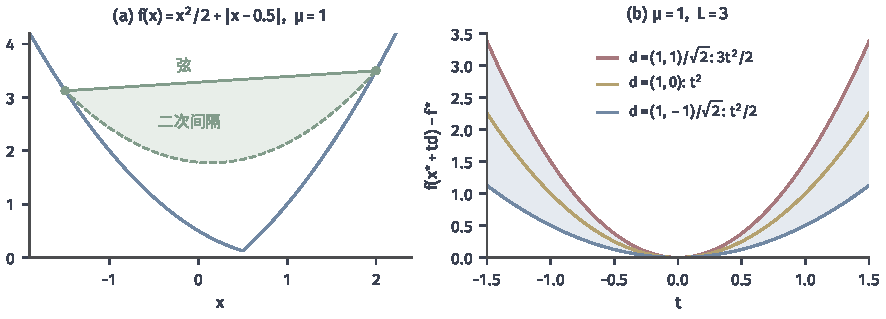
\includegraphics[width=150mm]{figures/03-optimization-evolution-and-signals/01-optimization/matplotlib/c1-strong-convex-gap/figure.pdf}
  \caption{强凸性的二次间隔。(a) $f(x)=x^2/2+|x-0.5|$是$1$强凸的：连接$u=-1.5$与$v=2$的绿色弦下方，虚线是弦减去$\frac{1}{2}\theta(1-\theta)(u-v)^2$，函数图像（蓝）始终不高于虚线，浅绿区域是强凸性保证的间隔。(b) 最小二乘实例取$\lambda=1$，$\bm H=\begin{pmatrix}2&1\\1&2\end{pmatrix}$，特征值为$1$与$3$；沿三个单位方向$\bm d$画出$f(\bm x^\star+t\bm d)-f^\star=\frac12t^2\bm d^\top\bm H\bm d$，所有曲线都夹在$\frac12t^2$与$\frac32t^2$之间（浅蓝带）。}
  \label{fig:opt-prob-strong-convex-gap}
\end{figure*}

\paragraph{目标差控制到最小点的距离}
强凸性最直接的用途，是把目标值的误差换成参数的误差。

\begin{theorem}[强凸目标的二次增长]
\label{thm:opt-prob-strong-growth}
设$C$为凸集，$f$在$C$上关于范数$\lVert\cdot\rVert$为$\mu$强凸，且$\bm x^\star\in\argmin_{\bm x\in C}f$存在。则对所有$\bm x\in C$，
\begin{equation}
  f(\bm x)-f^\star\geq\frac{\mu}{2}\lVert\bm x-\bm x^\star\rVert^2,
  \qquad\text{从而}\qquad
  \lVert\bm x-\bm x^\star\rVert\leq\sqrt{\frac{2\bigl(f(\bm x)-f^\star\bigr)}{\mu}}.
  \label{eq:opt-prob-quadratic-growth}
\end{equation}
特别地，最优解唯一。
\end{theorem}

\begin{proof}
对$t\in(0,1)$，点$\bm x^\star+t(\bm x-\bm x^\star)$在$C$中，其目标值不低于$f^\star$。在式~\eqref{eq:opt-prob-strong-convexity}中取$\bm u=\bm x$、$\bm v=\bm x^\star$、$\theta=t$：
\[
  f^\star\leq f\bigl(\bm x^\star+t(\bm x-\bm x^\star)\bigr)\leq tf(\bm x)+(1-t)f^\star-\frac{\mu}{2}t(1-t)\lVert\bm x-\bm x^\star\rVert^2.
\]
整理并除以$t>0$，得$f(\bm x)-f^\star\geq\frac{\mu}{2}(1-t)\lVert\bm x-\bm x^\star\rVert^2$；令$t\downarrow0$即得式~\eqref{eq:opt-prob-quadratic-growth}。若$\bm x$也是最优解，左端为零，迫使$\bm x=\bm x^\star$。
\end{proof}

证明只用到可行域凸、目标强凸和最小点存在，没有假设最小点在内部或目标可微，所以对约束问题与非光滑目标同样成立。以实例$\lambda=1$为例，$\bm x^\star=(2/3,2/3)$，$\mu=1$。取$\bm x=\bm x^\star+(1,-1)=(5/3,-1/3)$，由于最优点处梯度为零，二次函数的展开给出$f(\bm x)-f^\star=\frac12(1,-1)\bm H(1,-1)^\top=1$；式~\eqref{eq:opt-prob-quadratic-growth}给出距离上界$\sqrt{2\cdot1/1}=\sqrt2$，恰好等于实际距离，因为位移方向正是最小特征值的特征向量。

\paragraph{曲率下界与曲率上界}
图~\ref{fig:opt-prob-strong-convex-gap}(b)展示了同一个二次函数沿不同方向离开最小点时的增长。无约束且$\nabla f(\bm x^\star)=\bm 0$时，$f(\bm x)-f^\star=\frac12(\bm x-\bm x^\star)^\top\bm H(\bm x-\bm x^\star)$，因此
\[
  \frac{\lambda_{\min}(\bm H)}{2}\lVert\bm x-\bm x^\star\rVert_2^2\leq f(\bm x)-f^\star\leq\frac{\lambda_{\max}(\bm H)}{2}\lVert\bm x-\bm x^\star\rVert_2^2.
\]
下界来自强凸常数$\mu$，它说明目标差小时参数不可能离得太远；上界来自曲率的上限，它说明参数接近时目标差也小。对一般函数，上界对应梯度的Lipschitz常数$L$，第~\ref{chap:opt-smooth}章将系统使用$L$与$\mu$及其比值$\kappa=L/\mu$。两个常数回答的是相反方向的问题，不能互相替代。

\paragraph{可行域必须凸}
定理~\ref{thm:opt-prob-strong-growth}要求可行域凸，这一条件不能省略。$f(x)=x^2$在$\mathbb R$上$2$强凸，但在非凸集$C=\{x:|x|\geq1\}$上有两个最小点$\pm1$。取$\bm x^\star=-1$与$x=1$，目标差为$0$，距离却是$2$，式~\eqref{eq:opt-prob-quadratic-growth}不成立：证明中从$\bm x^\star$走向$\bm x$的线段离开了可行域。后续各章只在确有凸可行域与相应常数时才使用这类误差换算。

\section{光滑目标的最优条件}
\label{sec:opt-prob-optimality}

前两节的条件是几何的：可行域是否紧、目标是否凸。要真正判断某个候选是不是最优，我们需要能在这一点上计算的条件。目标可微时，多元微积分把函数在一点附近写成梯度项、Hessian二次型与高阶余项之和，这些局部量就成了判别工具。本节只处理可行域内部的点，等价于在该点附近做无约束比较；边界上的最优条件需要可行方向与乘子，留给第~\ref{chap:constrained-optimization}章。卷一已经从多元函数的角度建立了极值的一阶、二阶条件（可参考\BookChapterRef{chap:multivariate-calculus}{卷一“多元函数微分”章}），这里从优化的角度重新组织它们：哪些是必要条件，哪些是充分条件，什么时候局部判据能推出全局结论。

\subsection{一阶条件与驻点}
\label{sec:opt-prob-first-order}

\paragraph{沿每个方向看}
站在最低点上，朝任何方向迈一小步都不会更低。把这句话变成计算：固定方向$\bm d$，只看沿直线$\bm x^\star+t\bm d$的一元函数$\phi(t)=f(\bm x^\star+t\bm d)$。若$\bm x^\star$是局部最优解且在可行域内部，$\phi$在$t=0$处有局部最小，它的导数$\phi'(0)=\langle\nabla f(\bm x^\star),\bm d\rangle$不能为负；对$-\bm d$同样如此，于是它只能为零。

\begin{theorem}[一阶必要条件]
\label{thm:opt-prob-first-order-necessary}
设$\bm x^\star$是$C$的内点，即存在$r>0$使$B(\bm x^\star,r)\subseteq C$；$f$在$\bm x^\star$处可微。若$\bm x^\star$是$f$在$C$上的局部最优解，则$\nabla f(\bm x^\star)=\bm 0$。
\end{theorem}

\begin{proof}
对任意$\bm d$，$|t|$充分小时$\bm x^\star+t\bm d\in C\cap B(\bm x^\star,r')$，其中$r'$是局部最优的邻域半径。于是$\phi(t)=f(\bm x^\star+t\bm d)\geq\phi(0)$。当$t>0$时，$(\phi(t)-\phi(0))/t\geq0$，令$t\downarrow0$得$\langle\nabla f(\bm x^\star),\bm d\rangle\geq0$。以$-\bm d$代替$\bm d$得相反不等式，所以$\langle\nabla f(\bm x^\star),\bm d\rangle=0$对所有$\bm d$成立，取$\bm d=\nabla f(\bm x^\star)$即得梯度为零。
\end{proof}

梯度为零的点称为\term{驻点}（stationary point）。一阶条件只是必要条件，它的局限有三方面。第一，驻点不一定是最小点：$-\lVert\bm x\rVert_2^2$在原点有驻点，那里是最大点；$x^2-y^2$在原点也有驻点，沿$x$轴是最低点、沿$y$轴是最高点，这样的驻点称为\term{鞍点}（saddle point）。第二，定理只对内点成立：示例~\ref{ex:opt-prob-local-global}中，$C=[-1.5,1.5]$上的全局最优解$x=1.5$在边界上，导数是$-1.875$而不是零。第三，即使驻点是局部最优，也不一定是全局最优：同一函数在$x=-1$处导数为零且是局部最优，却比$C$上的最优值高得多。

\paragraph{凸目标的驻点是全局最优}
凸性把这个必要条件变成充分条件。若$f$在开凸集$D$上凸且可微，$\nabla f(\bm x^\star)=\bm 0$，代入一阶支撑下界~\eqref{eq:opt-prob-first-order-support}，对任意$\bm v\in D$，
\[
  f(\bm v)\geq f(\bm x^\star)+\langle\bm 0,\bm v-\bm x^\star\rangle=f(\bm x^\star).
\]

\begin{theorem}[凸目标驻点的全局最优性]
\label{thm:opt-prob-convex-stationary}
设$D$是开凸集，$f:D\to\mathbb R$凸且可微。则$\bm x^\star\in D$是$f$在$D$上的全局最优解，当且仅当$\nabla f(\bm x^\star)=\bm 0$。
\end{theorem}

必要性来自定理~\ref{thm:opt-prob-first-order-necessary}（开集中每点都是内点），充分性就是上面的一行计算。几何上，切平面是全局下界，水平的切平面就把最小值钉在了切点上。

这个结论的价值在于：对凸目标，求解优化问题等价于解方程$\nabla f=\bm 0$，并且找到的任何一个解都是全局最优。最小二乘的梯度为$\nabla f(\bm x)=\bm A^\top(\bm A\bm x-\bm b)+\lambda\bm x$，驻点条件就是正规方程$(\bm A^\top\bm A+\lambda\bm I)\bm x=\bm A^\top\bm b$。在实例中$\lambda=0$时，它化为$x_1+x_2=2$，与第~\ref{sec:opt-prob-local-global}小节由直接比较得到的最优解集合完全一致。

对非凸目标，找到驻点只能说明这一点附近没有一阶下降方向。它可能是局部最优、局部最大或鞍点；即使是局部最优，也可能远不是全局最优。这一区别在后续章节始终要保持：说一个方法“收敛到驻点”与说它“找到最优解”，是两个不同强度的结论。

\subsection{二阶条件与曲率}
\label{sec:opt-prob-second-order}

一阶条件无法区分极小、极大与鞍点，因为在驻点处梯度项消失了，函数的变化由下一阶的Hessian二次型主导。设$f$在$\bm x^\star$附近二阶连续可微，$\nabla f(\bm x^\star)=\bm 0$，记$\bm H=\nabla^2f(\bm x^\star)$。沿方向$\bm d$，
\[
  f(\bm x^\star+t\bm d)-f(\bm x^\star)=\frac{t^2}{2}\bm d^\top\bm H\bm d+o(t^2).
\]
$\bm d^\top\bm H\bm d$是函数沿$\bm d$方向的曲率：为正时向上弯，为负时向下弯。

\begin{theorem}[二阶条件]
\label{thm:opt-prob-second-order}
设$\bm x^\star$是$C$的内点，$f$在$\bm x^\star$附近二阶连续可微。
\begin{enumerate}
  \item （必要条件）若$\bm x^\star$是局部最优解，则$\nabla f(\bm x^\star)=\bm 0$且$\nabla^2f(\bm x^\star)$半正定。
  \item （充分条件）若$\nabla f(\bm x^\star)=\bm 0$且$\nabla^2f(\bm x^\star)$正定，则$\bm x^\star$是严格局部最优解。
\end{enumerate}
\end{theorem}

\begin{proof}
(1) 一阶部分即定理~\ref{thm:opt-prob-first-order-necessary}。若某个$\bm d$使$\bm d^\top\bm H\bm d<0$，上面的展开表明$t\neq0$充分小时$f(\bm x^\star+t\bm d)<f(\bm x^\star)$，与局部最优矛盾。

(2) 设$\bm H$正定，令$\lambda_{\min}>0$为其最小特征值，则$\bm h^\top\bm H\bm h\geq\lambda_{\min}\lVert\bm h\rVert_2^2$。由二阶Taylor公式与Hessian的连续性，可取$r>0$使$\lVert\bm h\rVert_2<r$时余项的绝对值不超过$\frac{\lambda_{\min}}{4}\lVert\bm h\rVert_2^2$，于是
\[
  f(\bm x^\star+\bm h)-f(\bm x^\star)\geq\frac{\lambda_{\min}}{2}\lVert\bm h\rVert_2^2-\frac{\lambda_{\min}}{4}\lVert\bm h\rVert_2^2=\frac{\lambda_{\min}}{4}\lVert\bm h\rVert_2^2>0
\]
余项估计的细节见卷一多元Taylor公式。
\end{proof}

回到示例~\ref{ex:opt-prob-local-global}：$f''(x)=3x^2-2x-2$，$f''(-1)=3>0$，$f''(2)=6>0$，二者都是严格局部最优；$f''(0)=-2<0$，$x=0$是局部最大点。二阶条件确认了图~\ref{fig:opt-prob-local-global}中所见的形状，但仍然只是局部结论，不能告诉我们$-1$与$2$哪个更低。

\paragraph{退化驻点}
两个条件之间留有缺口：Hessian半正定但奇异时，必要条件满足而充分条件不满足，二阶信息不足以判断。这样的驻点称为\term{退化驻点}（degenerate stationary point）。图~\ref{fig:opt-prob-stationary-types}的后两幅给出了缺口两侧的例子。$x^2+y^4$与$x^2+y^3$在原点的梯度都为零，Hessian都是$\operatorname{diag}(2,0)$，二阶信息完全相同。前者对$(x,y)\neq\bm 0$恒为正，原点是严格最小点，说明正定不是必要的；后者沿$(0,-t)$取值$-t^3<0$，原点不是局部最小点，说明半正定不是充分的。决定结果的是$y$方向上的高阶项，这正是Hessian在零特征方向上看不到的信息。

\begin{figure*}[!htbp]
  \centering
  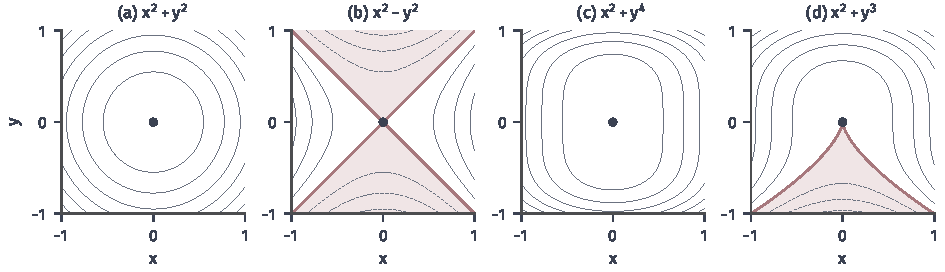
\includegraphics[width=160mm]{figures/03-optimization-evolution-and-signals/01-optimization/matplotlib/c1-stationary-types/figure.pdf}
  \caption{原点处四种驻点的等值线。灰线是等值线（虚线为负值），红色区域是函数值低于$f(\bm 0)=0$的点，红线是零等值线。(a) $x^2+y^2$：Hessian正定，严格最小点，附近没有更低的点。(b) $x^2-y^2$：Hessian不定，鞍点，红色区域从上下两侧伸到原点。(c) $x^2+y^4$：Hessian为$\operatorname{diag}(2,0)$，仍是严格最小点。(d) $x^2+y^3$：Hessian同为$\operatorname{diag}(2,0)$，但原点下方有更低的点，不是最小点。}
  \label{fig:opt-prob-stationary-types}
\end{figure*}

读者应从图中注意红色区域是否碰到原点：碰到就说明任意小的邻域里都有更低的点。(c)与(d)的二阶信息相同，红色区域却一有一无。

\paragraph{负曲率方向}
定理~\ref{thm:opt-prob-second-order}的必要性证明还包含一个可操作的信息。若驻点处存在方向$\bm d$使$\bm d^\top\nabla^2f(\bm x^\star)\bm d<0$，称$\bm d$为\term{负曲率方向}（negative curvature direction）。沿这个方向，一阶变化为零，函数却以$\frac{t^2}{2}\bm d^\top\bm H\bm d$的速度下降。图~\ref{fig:opt-prob-saddle-curvature}以$f(x,y)=x^2-y^2$为例：沿$(1,0)$方向函数向上弯，沿$(0,1)$方向向下弯，沿$(1,1)/\sqrt2$方向二阶项恰好为零。站在鞍点上，梯度不会指出任何下降方向，Hessian的负特征向量却指出了一条。第~\ref{chap:opt-smooth}章将利用这一判断讨论怎样离开鞍点。

\begin{figure*}[!htbp]
  \centering
  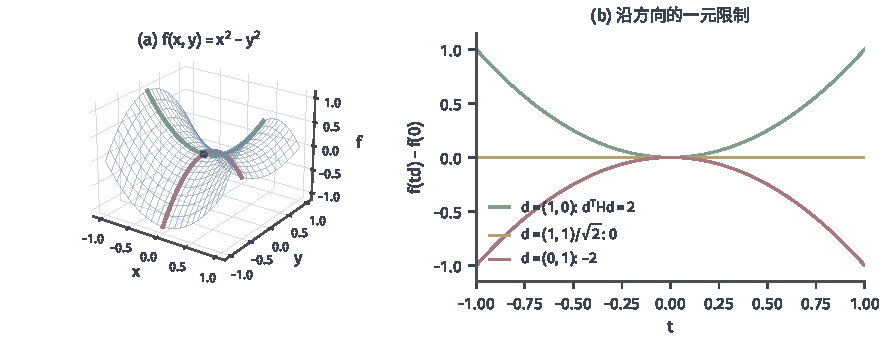
\includegraphics[width=150mm]{figures/03-optimization-evolution-and-signals/01-optimization/matplotlib/c1-saddle-curvature/figure.pdf}
  \caption{鞍点与负曲率方向。(a) 曲面$f(x,y)=x^2-y^2$，绿色曲线是沿$x$轴的截线（向上弯），红色曲线是沿$y$轴的截线（向下弯），黑点是驻点$\bm 0$。(b) 沿单位方向$\bm d$的一元限制$f(t\bm d)-f(\bm 0)=t^2\bm d^\top\bm H\bm d/2$，其中$\bm H=\operatorname{diag}(2,-2)$：方向$(1,0)$曲率为$2$，$(1,1)/\sqrt2$为$0$，$(0,1)$为$-2$，后者是负曲率方向。}
  \label{fig:opt-prob-saddle-curvature}
\end{figure*}

把本节与上一节合起来看：对一般光滑目标，梯度为零、Hessian正定只给出局部结论；对凸目标，梯度为零已经给出全局结论；对强凸目标，全局最优解还唯一，并且目标差控制到它的距离。条件越强，局部计算能推出的结论越强。

\section{近似解与计算评价}
\label{sec:opt-prob-approximation}

前四节讨论的是精确的最优解。实际计算几乎从不交出精确解：迭代在有限步后停止，浮点运算带来舍入，数据本身也有误差。于是需要回答一个新问题：在给定预算内得到的结果，好到什么程度？这个问题有两个维度。结果误差规定“有多准”，计算成本规定“为此付出多少”。本节为后续各章建立共同的评价语言；具体的误差界、停止规则和误差传播，随相应方法在各章展开。

\subsection{目标误差、解误差与最优性残差}
\label{sec:opt-prob-error-measures}

\paragraph{三种误差}
设$\hat{\bm x}\in C$是交出的可行近似解，最优值$f^\star$有限，最优解集合$S=\argmin_{\bm x\in C}f$非空。至少有三种量可以衡量它的好坏。

\begin{itemize}
  \item 目标差$f(\hat{\bm x})-f^\star\geq0$：结果比最优值差多少。若$f(\hat{\bm x})-f^\star\leq\varepsilon$，称$\hat{\bm x}$为目标值意义下的$\varepsilon$近似解。
  \item 到解集的距离$\operatorname{dist}(\hat{\bm x},S)=\inf_{\bm x\in S}\lVert\hat{\bm x}-\bm x\rVert_2$：参数离最优解有多远。最优解唯一时就是$\lVert\hat{\bm x}-\bm x^\star\rVert_2$。
  \item \term{最优性残差}（optimality residual）：在$\hat{\bm x}$处可以直接计算、并在最优解处为零的量。对无约束可微问题，最常用的是梯度范数$\lVert\nabla f(\hat{\bm x})\rVert_2$。
\end{itemize}

前两种量都含有未知的$f^\star$或$S$，求解过程中通常算不出来；第三种量能算，但它与前两者的关系需要额外条件。三者不能互相代替。

\paragraph{平坦目标中小梯度不等于小误差}
图~\ref{fig:opt-prob-flat-gradient}(a)比较两个一元二次函数$f_1(x)=0.01x^2/2$与$f_2(x)=x^2/2$，最小点都是$0$，最优值都是$0$。在$x=10$处$f_1'(10)=0.1$，在$x=0.1$处$f_2'(0.1)=0.1$，两个点的梯度一样小。但前者的目标差是$0.5$、到最小点的距离是$10$，后者分别是$0.005$和$0.1$，相差两个数量级。原因在于曲率：$f_1$的二阶导数只有$0.01$，地形太平，坡度很小时离谷底仍然很远。

\begin{figure*}[!htbp]
  \centering
  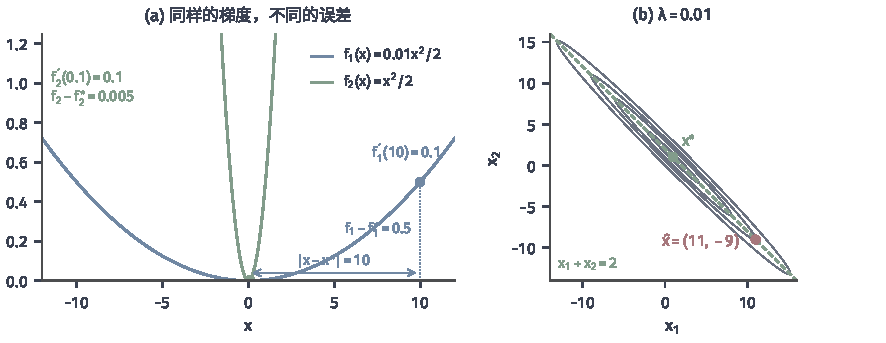
\includegraphics[width=150mm]{figures/03-optimization-evolution-and-signals/01-optimization/matplotlib/c1-flat-gradient/figure.pdf}
  \caption{小梯度与小误差。(a) 平坦的$f_1(x)=0.01x^2/2$（蓝）在$x=10$处与陡峭的$f_2(x)=x^2/2$（绿）在$x=0.1$处有相同的导数$0.1$，但$f_1$的目标差为$0.5$、到最小点的距离为$10$，$f_2$分别只有$0.005$和$0.1$。(b) 最小二乘实例取$\lambda=0.01$，灰线是$f-f^\star=0.1,0.5,1,2$的等值线，沿绿色虚线$x_1+x_2=2$极度拉长。$\hat{\bm x}=(11,-9)$（红点）的观测残差为零、梯度范数约$0.142$，但目标差约为$1.00$，到$\bm x^\star\approx(0.995,0.995)$的距离约为$14.1$。}
  \label{fig:opt-prob-flat-gradient}
\end{figure*}

\paragraph{小观测误差不等于小参数误差}
最小二乘实例给出多维的版本。先取$\lambda=0$。点$\hat{\bm x}=(11,-9)$满足$11+(-9)=2$，观测残差$\bm A\hat{\bm x}-\bm b=0$，它本身就是一个最优解，到最优解集合的距离为$0$。但如果我们心里的“正确参数”是$(1,1)$，两者相距$\lVert(10,-10)\rVert_2\approx14.1$。可见在解不唯一时，“参数误差”必须说明参照的是解集合还是某个指定的解；观测拟合得再好，也不能告诉我们数据没有约束的方向。

再取$\lambda=0.01$，问题有唯一解$\bm x^\star=\frac{2}{2.01}(1,1)\approx(0.995,0.995)$，最优值$f^\star=\frac{0.01\cdot4}{2\cdot2.01}\approx0.00995$。对同一个$\hat{\bm x}=(11,-9)$，观测残差仍为零，梯度$\nabla f(\hat{\bm x})=\bm A^\top(\bm A\hat{\bm x}-\bm b)+\lambda\hat{\bm x}=(0.11,-0.09)$，范数约为$0.142$；目标值$f(\hat{\bm x})=0.005\cdot(121+81)=1.01$，目标差约为$1.00$；到$\bm x^\star$的距离约为$14.1$。图~\ref{fig:opt-prob-flat-gradient}(b)显示了原因：强凸常数$\mu=\lambda=0.01$很小，等值线沿$(1,-1)$方向被拉得极长，$\hat{\bm x}$虽在谷底的“长沟”里，却离真正的最低点很远。

\paragraph{残差何时能控制误差}
强凸性给出了从残差到误差的换算。设$f$在$\mathbb R^d$上可微且$\mu$强凸。在式~\eqref{eq:opt-prob-strong-first-order}中取$\bm u=\hat{\bm x}$，右端是$\bm v$的二次函数，它在$\bm v=\hat{\bm x}-\nabla f(\hat{\bm x})/\mu$处取得最小值$f(\hat{\bm x})-\lVert\nabla f(\hat{\bm x})\rVert_2^2/(2\mu)$，所以对所有$\bm v$，$f(\bm v)$都不低于这个数，特别地对$\bm v=\bm x^\star$：
\[
  f(\hat{\bm x})-f^\star\leq\frac{\lVert\nabla f(\hat{\bm x})\rVert_2^2}{2\mu}.
\]
再结合定理~\ref{thm:opt-prob-strong-growth}，又得$\lVert\hat{\bm x}-\bm x^\star\rVert_2\leq\lVert\nabla f(\hat{\bm x})\rVert_2/\mu$。代入上面的数值：$0.142^2/(2\cdot0.01)\approx1.01$，确实不小于实际目标差$1.00$；$0.142/0.01\approx14.2$，确实不小于实际距离$14.1$。两个界都成立且接近实际值，但它们都被$1/\mu$放大：$\mu$越小，同样大小的梯度允许越大的误差。没有$\mu$这样的常数，小梯度不能推出任何关于目标差或距离的结论；这正是图~\ref{fig:opt-prob-flat-gradient}要说明的。

\paragraph{实验评价与停止判据}
要区分两种使用场合。在实验评价中，我们常对同一问题先用高精度方法（例如直接解正规方程）算出参照最优值$f^\star$或参照解，再画出目标差或距离随计算量的变化；这适合比较方法，但参照值本身也有误差，应当说明它是怎样得到的。在实际求解中，$f^\star$未知，只能依据可计算的残差决定何时停止，例如“梯度范数低于$\varepsilon$”；它对目标差的含义取决于是否有$\mu$这类条件。约束问题还要同时检查约束违背程度，非光滑问题要用替代梯度的量，而对偶间隙能直接给出目标差的上界；这些残差分别在第~\ref{chap:opt-nonsmooth}章与第~\ref{chap:constrained-optimization}章建立后才能使用，本章不提前使用它们。

\subsection{迭代次数与总计算成本}
\label{sec:opt-prob-cost}

\paragraph{先固定比较的对象}
后续章节的方法都产生一列迭代$\bm x^{(t)}$，$t=0,1,2,\dots$，并用某个误差$e^{(t)}\geq0$描述第$t$轮的质量。$e^{(t)}$可以是目标差、到解集的距离，也可以是某种残差；比较两个方法前，必须先说清比较的是哪一个。上面的例子已经表明，三者可以相差几个数量级。

\paragraph{三类收敛结论}
关于$e^{(t)}$的结论有强弱之分。
\begin{itemize}
  \item 渐近收敛：$e^{(t)}\to0$。它只说最终会任意准，不说要多少轮。
  \item 有限步误差界：对所有$t$都有可计算的上界$e^{(t)}\leq B(t)$。若$B(t)=c/(t+1)$之类按幂次下降，称为\term{次线性收敛}（sublinear convergence）；若$B(t)=c\rho^t$，$0<\rho<1$，称为\term{线性收敛}（linear convergence），在对数坐标中是一条直线。
  \item 局部收敛阶：若$e^{(t)}\to0$，且存在$M>0$、$p>1$，使$t$充分大后$e^{(t+1)}\leq M(e^{(t)})^p$，称收敛阶为$p$；$p=2$时称为\term{二次收敛}（quadratic convergence）。这类结论通常只在解的附近成立，不说明从远处出发要走多久。
\end{itemize}

由这些结论可以反推达到精度$\varepsilon$所需的轮数。线性收敛$c\rho^t\leq\varepsilon$需要$t\geq\log(c/\varepsilon)/\log(1/\rho)$，与$\log(1/\varepsilon)$成正比；次线性的$c/(t+1)\leq\varepsilon$需要约$c/\varepsilon$轮；二次收敛从$e^{(0)}=0.5$、$M=1$出发有$e^{(t)}=0.5^{2^t}$，只需约$\log_2\log_2(1/\varepsilon)$轮。图~\ref{fig:opt-prob-convergence-cost}(a)画出了三条由公式生成的误差序列：$1/(t+1)$、$0.9^t$与$e^{(t+1)}=(e^{(t)})^2$。要达到$\varepsilon=10^{-8}$，它们分别需要约$10^8$轮、$175$轮与$5$轮。收敛速率的这些定义沿用数值优化的通行用法\scite{math-nocedal2006numerical}。

\paragraph{每轮代价}
轮数只是一半。每一轮要做什么、花多少，取决于方法使用的计算单元。常见的单元有：求一次函数值，求一次梯度，做一次矩阵向量乘积，或者精确求解一个子问题。以稠密的$\bm A\in\mathbb R^{n\times d}$为例，最小二乘的一次函数值需要算$\bm A\bm x$，约$nd$次乘加；一次梯度$\bm A^\top(\bm A\bm x-\bm b)+\lambda\bm x$需要两次矩阵向量乘积，约$2nd$次乘加；若要直接解正规方程，形成$\bm A^\top\bm A$约需$nd^2$次乘加的量级，再对$d\times d$矩阵作Cholesky分解约需$d^3/3$次运算的量级。存储量也要登记：存$\bm A$需要$nd$个数，存$\bm A^\top\bm A$需要$d^2$个数。

\paragraph{总成本}
把两部分合起来，
\[
  \text{总成本}\approx\text{准备代价}+\text{每轮代价}\times\text{达到精度}\ \varepsilon\ \text{所需的轮数}.
\]
图~\ref{fig:opt-prob-convergence-cost}(b)把(a)中的线性序列和二次序列改按累计代价画出，假设前者每轮代价为$1$、后者为$40$。按轮数看，二次序列遥遥领先；按总代价看，达到$10^{-8}$时线性序列花$175$、二次序列花$5\times40=200$，前者反而更省；要求提高到$10^{-12}$时，二次序列只需$6$轮共$240$，线性序列需要$263$，二者又调换了位置。哪一个更划算，同时取决于精度要求和每轮代价。

\begin{figure*}[!htbp]
  \centering
  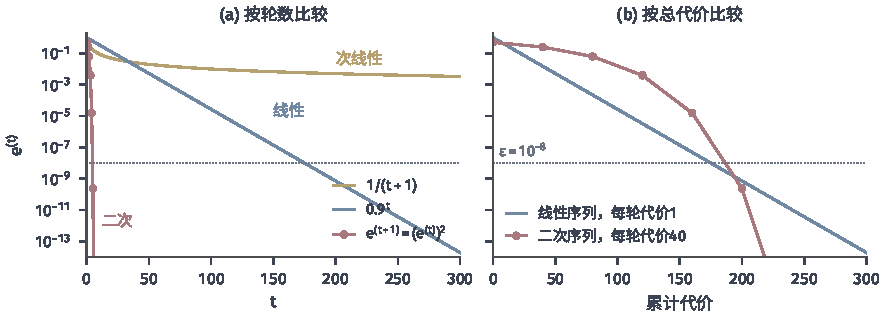
\includegraphics[width=150mm]{figures/03-optimization-evolution-and-signals/01-optimization/matplotlib/c1-convergence-cost/figure.pdf}
  \caption{收敛速率与总代价。三条曲线是由公式生成的误差序列，不是某个算法的实测结果，纵轴为对数刻度，灰色点线标出$\varepsilon=10^{-8}$。(a) 按轮数：次线性$1/(t+1)$（黄）、线性$0.9^t$（蓝）、二次$e^{(t+1)}=(e^{(t)})^2$且$e^{(0)}=0.5$（红）。(b) 按累计代价：线性序列每轮代价$1$，二次序列每轮代价$40$；达到$10^{-8}$分别需要$175$与$200$，达到$10^{-12}$分别需要$263$与$240$。}
  \label{fig:opt-prob-convergence-cost}
\end{figure*}

这给后续各章立下一条比较规则：比较两个方法时，应采用相同的问题、相同的误差对象、相同的精度要求和相同的输入规模，把每轮代价与轮数一起报告，必要时登记存储量。“二阶方法”“加速方法”这样的名称描述的是更新的构造方式，不能直接断定总效率更高；第~\ref{chap:opt-smooth}章起，每个方法都按这一口径给出输入、每轮代价与误差界。

\section{本章小结}
\label{sec:opt-prob-summary}

章首把优化想象成在一块允许站的地上找最低点。本章把这幅画面拆成了几个分别回答的问题。问题的表述要同时给出决策变量、目标函数与可行域；最优值是下确界，最优解是取得它的可行点，二者可以分离：问题可能不可行、无下界，或最优值有限却未达到。局部最优只与附近的可行点比较，全局最优与所有可行点比较；扩展实值写法用指示函数把约束并入目标，不改变最优值与最优解，而有限惩罚会改变问题。

两个贯穿例子展示了这些问题怎样得到回答。资源分配的可行域是有界多面体，紧集上的连续目标保证最优解存在；把两条资源约束相加，就同时得到利润上界$10$和达到它的方案$(2,2)$。最小二乘的可行域无界，正则项$\lambda>0$使目标强制，从而最优解存在；同一个正则项使Hessian$\bm A^\top\bm A+\lambda\bm I$正定，目标严格凸乃至$\lambda$强凸，于是最优解唯一，目标差还能换成到最优解的距离。$\lambda=0$且$\bm A$秩亏时，这些结论依次失效：目标不强制，最优解仍存在却成一条直线，参数不唯一而给定样本上的预测相同。

表~\ref{tab:opt-prob-summary}汇总了各个结论所需的条件。表中的条件都是充分条件，反例列说明去掉条件或反向推断时会出什么问题。

\begin{table*}[!htbp]
\centering
\caption{本章主要问题、充分条件与边界。表中“凸”均指可行域凸且目标凸；强凸常数$\mu$对应欧氏范数。}
\label{tab:opt-prob-summary}
\small
\begin{tabularx}{\linewidth}{@{}>{\RaggedRight\arraybackslash}p{24mm}>{\RaggedRight\arraybackslash}X>{\RaggedRight\arraybackslash}X>{\RaggedRight\arraybackslash}X@{}}
\toprule
问题 & 充分条件 & 结论 & 反例或边界 \\
\midrule
最优解是否存在 & 可行域非空紧，目标适当且下半连续；或可行域非空闭，目标适当、下半连续且强制 & 最优值有限且被达到 & $(0,1]$上的$x$；$[1,\infty)$上的$1/x$；在$0$处跳高的函数；无限维中有界闭集不紧 \\
局部是否即全局 & 凸 & 每个局部最优解都是全局最优解，最优解集合凸 & $x^4/4-x^3/3-x^2$在$x=-1$处的局部最优 \\
最优解是否唯一 & 凸可行域上严格凸，且最优解存在 & 最优解唯一 & $e^x$严格凸而无最小点；$|x|$与资源分配问题有唯一解而目标不严格凸 \\
目标差能否换成距离 & 凸可行域上$\mu$强凸，且最优解存在 & $f(\bm x)-f^\star\geq\frac{\mu}{2}\lVert\bm x-\bm x^\star\rVert^2$ & 非凸可行域$\{|x|\geq1\}$上的$x^2$ \\
内点能否用梯度判别 & 可微；凸目标在开凸集上 & 局部最优必有$\nabla f=\bm 0$；凸时$\nabla f=\bm 0$即全局最优 & 鞍点$x^2-y^2$；边界最优点导数可不为零 \\
驻点是否局部最优 & 二阶连续可微，Hessian正定 & 严格局部最优解 & $x^2+y^4$（正定非必要）；$x^2+y^3$（半正定不充分） \\
小残差是否表示小误差 & 可微且$\mu$强凸 & $f(\hat{\bm x})-f^\star\leq\lVert\nabla f(\hat{\bm x})\rVert_2^2/(2\mu)$ & 平坦目标$0.01x^2/2$；$\lambda=0.01$的最小二乘 \\
\bottomrule
\end{tabularx}
\end{table*}

最后一节说明了怎样评价实际交出的近似解。目标差、到解集的距离与可计算的残差是三种不同的误差，只有在强凸这类附加条件下才能互相换算，换算系数随$1/\mu$放大。比较方法时，还要把达到指定精度的轮数与每轮代价合成为总成本，并在相同的问题、误差对象、精度和规模下比较。

本章没有生成任何迭代序列，也没有假设任何算法已经成功。我们得到的是后续各章共同使用的语言：有限维的凸几何、解的存在与唯一、内点的最优条件，以及评价近似解的口径。下一章在最具体的线性模型上把这些语言用于一个完整的求解过程：可行域是多面体，最优解在顶点中寻找，而“把约束加权相加得到下界”的想法将发展为可以核对的最优性证书。

